\documentclass[12pt]{article}
\usepackage[margin = 1 in]{geometry}
\usepackage{amsmath, amsfonts, amssymb, graphicx, amsthm, quiver, hyperref}

\newcommand{\F}{\mathbf{F}}
\newcommand{\C}{\mathbb{C}}
\newcommand{\R}{\mathbb{R}}
\renewcommand{\P}{\mathbb{P}}
\newcommand{\GL}{\mathrm{GL}}
\newcommand{\A}{\mathbb{A}}
\newcommand{\Aff}{\mathrm{Aff}}
\renewcommand{\vec}{\overrightarrow}
\newcommand{\PGL}{\mathrm{PGL}}
\newcommand{\Res}{\mathrm{Res}}
\newcommand{\Z}{\mathbb{Z}}
\renewcommand{\S}{\mathbb{S}}
\newcommand{\Id}{\mathrm{Id}}
\newcommand{\Mor}{\mathrm{Mor}}
\newcommand{\id}{\mathrm{id}}
\newcommand{\Hom}{\mathrm{Hom}}
\newcommand{\m}{\mathfrak{m}}
\newcommand{\Frac}{\mathrm{Frac}}
\renewcommand{\O}{\mathcal{O}}
\renewcommand{\phi}{\varphi}

\newtheorem{fact}{Fact}[section]
\newtheorem{definition}{Definition}[section]
\newtheorem*{example}{Example}
\newtheorem{theorem}{Theorem}[section]
\newtheorem*{theorem*}{Theorem}
\newtheorem{proposition}{Proposition}[section]
\newtheorem{lemma}{Lemma}[section]

\title{Algebraic Geometry Notes}
\author{Raman Aliakseyeu}
\date{Winter 2024}

\begin{document}
    \maketitle
    \noindent \textbf{Course by Daniil Rudenko.} \par 
    We will start with projective geometry, and then add algebra to it. No schemes in this course, we will be closer to the 19th century stuff. We are not following any particular book(s). Number one book is "Algebraic Geometry" by Shafarevich, our goal is all of chapter 1. We will start with projective geometry, a book for that is Prasolov (roughly). 
    \section{Projective Geometry} 
    \subsection{Lecture 1} 
        Algebraic geometry studies solutions to systems of algebraic equations/algebraic curves (which are loci of solutions of algebraic equations). One of the most famous renaissance geometry results is the Pascal theorem: the points $G, H, I$ in the diagram below are colinear for any configuration of $A, B, C, D, E, F$ on the circle. 
        \begin{center}
            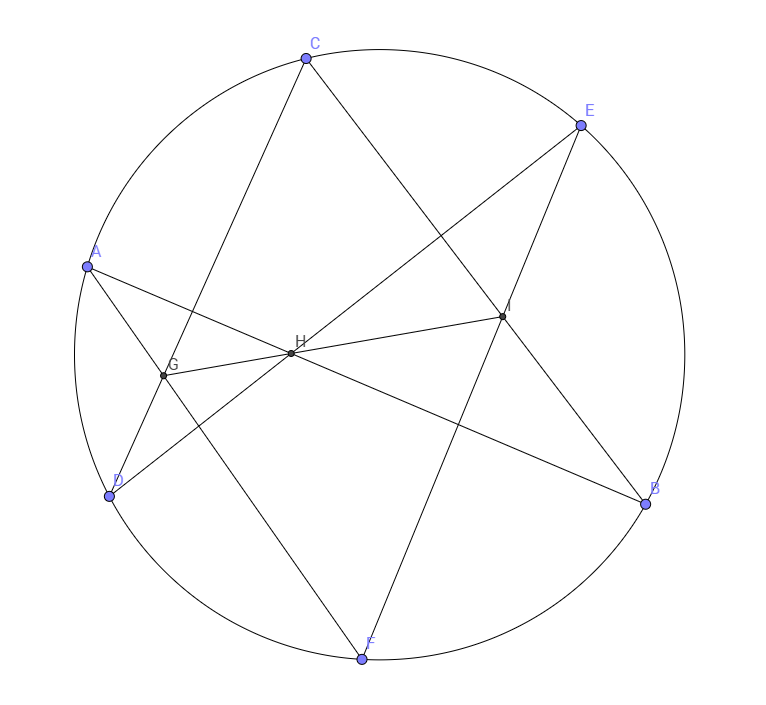
\includegraphics[width = 0.5 \linewidth]{pascals-theorem.PNG}
        \end{center}
        A similar result to that is Pappus' theorem. Another top theorem is by Cayley-Salman 1849: A smooth projective cubic surface contains exactly 27 lines. Another such theorem is that any smooth projective curve of degree 4 has 28 bitangent lines (tangent in exactly two points). Working toward proofs of these results using algebraic geometry is our goal. \par 
        \textit{History of the subject}: throughout the 19th century it developed very quickly, people who were into Euclidean geometry just transitioned to algebraic geometry and discover miracles like we described above. During the late 19th century Italians, who before led algebraic geometry, started producing very incorrect results because the technical aspects became too hard. Oscar Zariski and others saved the subject by rigorizing it using commutative algebra, with the language of ideals and rings, etc. We will see some `wrong' arguments by the Italian school and see why they are not precise enough. There was another revolution by Grothendieck and the Bourbaki group in developing the language of schemes, which we will not touch in this course (``You will need to sacrifice a year of your life to start speaking that language. I never needed to, but a lot of people do.'')\par 
        (Rudenko plug: woollymathematics.com)\par 
        Take $\F$ to be some field (usually $\C$), and polynomials $p_1, \dots, p_k \in \F[x_1, \dots, x_n]$, and study the solutions to the system 
        $$\begin{cases}
            p_1(x_1, \dots, x_n) = 0 \\
            \vdots \\
            p_k(x_1, \dots, x_n) = 0
        \end{cases}$$
        \begin{fact}
            If $k = 1$ and $p_1(x) = x^d + a_{d-1}x^{d-1} + \dots + a_0$ for $d \geq 1$, $p_1(x) = 0$ has $\leq d$ solutions in $\F$. 
        \end{fact}
        If $k = 2$, the number of solutions is $\leq$ than the product of the degrees of the polynomials. Of course we usually want a precise number of solutions, but generally we can't hope for anything more than upper bounds. 
        \begin{fact}
            If $\F = \C$, then $p(x) = 0$ has a solution. 
        \end{fact}
        This is a remarkably hard result called the Fundamental Theorem of Algebra. There is a result that is in a way easier:
        \begin{fact}
            If $\F = \C$, then $p(x) = 0$ has exactly $d$ solutions if counted with multiplicity. 
        \end{fact} 
        We would hope for something like that but for $k > 1$. Bezout's theorem kind of satisfies that, but the picture is more complicated. For example, take a line and a hyperbola. While we would expect $4$ solutions up to multiplicity, but take a line intersecting one of the components of the hyperbola transversally that is parallel to one of the other component's asymptotes. However, everything becomes nicer if we change the complex plane to the projective plane. The study of geometry on the projective plane is the projective geometry, and that's what we will study first. \par 
        \begin{definition} \label{def:proj_plane}
            Let $\F$ be a field. A \textbf{projective space} $\P_\F^n$ is the set of lines in the vector space $\F^{n+1}$. 
        \end{definition}
        An example for $\F = \R$, $\P_{\R}^2$ is the set of lines through the origin in the real plane. We can think of $\P_\R^1$ as all the points of a line in $\R^2$ not through the origin (say the line $y = 1$ in $\R^2$) but with a point at infinity added. \par 
        In $\R^2$, usually two lines intersect at one point, and two points are contained in one line. We can also define $\P_\R^2$ as the set of points of $\R^2$, and the set $[l]$ (points at $\infty$), which are equivalence classes of lines in $\R^2$ by $l_1 \sim l_2$ for $l_1$ and $l_2$ are parallel. Note that there is one more line, line at infinity, consisting only of points $[l]$. \par 
        \begin{fact}
            In $\P^2_\R$ every two distinct lines intersect in one point and every two points are contained in precisely one line. 
        \end{fact}
        \begin{proof}
            Non-parallel lines intersect in the usual way. Parallel lines intersect at their equivalence class $[l]$. If one of the lines is the `line at infinity', they intersect at the equivalence class of the other line. Similarly we can examine the second part of the statement. 
        \end{proof}
        \begin{fact}
            For $\P_\R^2$, the abstract definition \ref{def:proj_plane} is equivalent to the definition we gave in the example. 
        \end{fact}
        \begin{proof}
            Take a plane in $\R^3$ not passing through the origin, $z = -1$ for example. Then we can create a bijection between the set of lines through the origin and the set of points on the plane and the set of points at infinity, by mapping the lines that intersect the plane with their intersection point, and those that are parallel with the plane to their equivalence class on the plane $\R^2$. Thus we have a bijection between the two objects we defined. 
            \begin{center}
                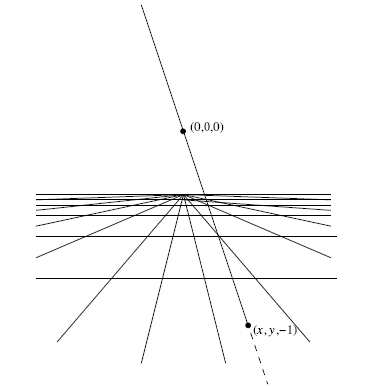
\includegraphics[width = 0.4\linewidth]{proj-plane.jpg}
            \end{center}
        \end{proof}
        Another way to think of $\P_\R^2$ is as a sphere with antipodal points identified. \par
        ``ChatGPT can make you Snake 4: Snake but on the projective plane.''
        
    \subsection{Lecture 2} 
    A \textbf{geometry} is a set $X$ along with a group $G$ acting on $X$, $x \mapsto gx$, which defines `equivalences' between subsets of $X$. 
    \begin{example}
        \begin{itemize}
            \item Let $X = \R^2$, $G$ the group of \textbf{isometries}: distance preserving bijections. Indeed, isometries also preserve lengths, areas, angles, etc. Think of them as congruences in Euclidean geometry. 
            \item Let $X$ be a vector space, $G = \text{GL}(V)$, the general linear group. More specifically, let $X = F^n$ for some field $G$, then $G = \GL_n(F)$.  
        \end{itemize}
    \end{example}
    \begin{definition}
        Fix $F$ some field. Define \textbf{affine space} $\A_F^n = F^n$, with the group of \textbf{affine transformations} $$\mathrm{Aff}_n = \{f: \A^n \to \A^n \mid f(x) = Ax + b, A \in \GL_n(F), b \in A^n\}$$
    \end{definition}
    A typical way of thinking about affine space is as a vector space without a fixed origin. 
    \begin{example}
        Circles don't make much sense in $\A_\R^2$ anymore, since $x^2 + y^2 = 1$ is equivalent to an ellipse (say by $(x, y) \mapsto (2x, 5y)$). 
    \end{example}
    \begin{definition}
        An \textbf{affine algebraic variety} is a set of solutions of a system of polynomials $P_1, \dots, P_k \in F[x_1, \dots, x_n]$:
        $$\begin{cases}
            P_1(x_1, \dots, x_n) = 0 \\
            \vdots \\
            P_k(x_1, \dots, x_n) = 0
        \end{cases}$$
    \end{definition}
    \begin{example}
        \begin{itemize}
            \item $P_1(x, y) = 2x + y - 1 = 0$ gives a line; $P_1(x, y) = x^2 + y^2 - 1 = 0$ gives a circle.
            \item $P_1(x, y, z) = 2x+y-z-1 = 0$ and $P_2(x, y, z) = x + y -3 = 0$, then the variety is an intersection of two planes, thus a line.  
        \end{itemize}
    \end{example}
    If $P_1, \dots, P_k$ are linear $\sum a_i x_i + b$ then we will call it \textbf{affine subspace}.\par 
    We can identify pairs of points in $\A^n$ with vectors in a vector space $F^n$, where vectors $\overrightarrow{AB}$ are pairs of points $(A, B)$, identified via the equivalence relation $\overrightarrow{A_1B_1} \sim \overrightarrow{A_2B_2}$ iff $(A_1)_i - (B_1)_i = (A_2)_i - (B_2)_i$. An observation is that if $f: \A^n \to \A^n$ is an affine transformation, then $f(\overrightarrow{AB}) = \overrightarrow{f(A)f(B)}$. \par 
    What we just described is a homomorphism $\mathrm{Aff}_n \to \GL_n$ which maps $f = Ax + b$ to $A \in \GL_n$. The kernel of this map is isomorphic to $\F^n$ as an additive group. \par 
    \begin{definition}
        If $A_1, \dots, A_{n+1} \in \A^n$ are in \textbf{general position} if $\overrightarrow{A_1A_i}$ for $i = 2, 3, \dots n+1$ are all linearly independent. Equivalently (exercise) $A_1, \dots, A_{n+1}$ are not in the same affine hyperplane. 
    \end{definition}
    \begin{theorem}
        Suppose $A_1, \dots, A_{n+1} \in \A^n$ and $B_1, \dots, B_n \in \A^n$ are points in general position in $\A^n$. Then there is a unique $f \in \Aff_n$ s.t. $f(A_i) = B_i$ for each $i$.  
    \end{theorem}
    \begin{proof}
        [Proof sketch:] Using translation by a vector $\overrightarrow{A_1B_1}$, move $A_1$ to $B_1$. This reduces this problem to the uniqueness of a linear transformation from the basis $\overrightarrow{A_1A_i} \to \overrightarrow{B_1B_i}$. 
    \end{proof}
    Observation: ``$X$ is the midpoint of the segment $\overline{A_1A_2}$'' is an affine property: $f(X)$ is still the midpoint of $\overline{f(A_1)f(A_2)}$. Application of this: 
    \begin{theorem}
        Three medians of a triangle intersect at a point. 
    \end{theorem} 
    \begin{proof}
        Let $ABC$ be an arbitrary triangle in $\A_\R^2$. Let $f$ be the affine transformation taking an equilateral triangle to $ABC$. The medians of an equilateral triangle intersect at a point by symmetry. But medians get sent to medians, and intersections are preserved, so the medians of $ABC$ must intersect also. 
    \end{proof}
    \begin{definition}
        Let $V$ be a vector space over $F$, then its \textbf{projectivization} $\P(V)$ is the set of lines (1-dim vector subspaces) in $V$. 
    \end{definition}
    By definition the dimension of $\P(V)$ is $\dim V - 1$. If $V = F^{n+1}$, $\P(V) = \P_F^n$. More explicitly, $\P(V) = (V - \{0\})/(v \sim \lambda v, \lambda \in F)$. 
    We express points in $\P(V)$ by \textbf{homogeneous coordinates} so $[X_0: X_1 : \dots : X_n]$, with the aforemetioned equivalence relation (so e.g. $[0, 1, 0] = [0, 2, 0]$) \par 
    ``Gold to silver to whiskey, the ratio should be 1 to 1 to 100. You're making a cocktail. Don't do that by the way... Point of projective geometry is to make cocktails.''\par 
    If $A = [X_0: \dots :X_n] \in \P^n$. If $X_n \neq 0$ then $A = [X_0/X_n: \dots : X_{n-1}/X_n, 1]$, points of this form this are in bijection with $\A^n$. The points with $X_n = 0$ are in bijection with points in $\A^{n-1}$ (divide all entrees by the first non-zero entry from the right). Indeed, $\P^n = \A^n \sqcup \A^{n-1} \sqcup \dots \sqcup \A^0$. For example, $\P_\R^1 = \R \cup \infty$, where $\R$ is in bijection with points $[X_0/X_1:1]$ and $\infty$ represents $[1:0]$.  \par 
    \textbf{Barycentric coordinates} are basically the same thing as homogeneous coordinates but in a different language. Imagine putting masses $m_1, m_2, m_3$ at the vertices of a triangle, then look at their center of mass. If $m_1 = m_2 = m_3$ then this point is the centroid. More precisely, if $O$ is any point, we have that the point $M$ with homogeneous coordinates $(m_1, m_2, m_3)$, the center of mass for some $m_1, m_2, m_3$ (sum non-zero), is such that
    $$\vec{OM} = \frac{m_1\vec{OA_1} + m_2\vec{OA_2} + m_3\vec{OA_3}}{m_1 + m_2 + m_3}$$
    As such, $M$ has homogeneous coordinates $(m_1:m_2:m_3)$ in the projective plane.  \par 
    A homogeneous polynomial is one where each term has the same degree. Then it makes sense to talk about $P([x_0, \dots, x_d]) = 0$ for a homogeneous polynomial $P$, since such polynomials respect the equivalence relation of homogeneous coordinates. 
    \begin{definition}
        \textbf{Projective variety} is a subset of $\P_F^n$ which is the set of solutions of a system:
        $$\begin{cases}
            P_1([X_0: \dots : X_n]) = 0 \\ 
            \vdots \\
            P_k([X_0: \dots : X_n]) = 0
        \end{cases}$$
        where each $P_i$ is homogeneous. 
    \end{definition}
    \begin{example}
        Say $P(x, y, z) = y - x^2$, which we can think of as points $[x:y:1]$ that satisfy the parabola. We can relabel $[x:y:1]$ into $[X:Y:Z]$ with $x = X/Z, y = Y/Z$, so the set of points satisfying $P_1([X:Y:Z])$ is the set such that $X^2 = YZ$. So for instance $[0:1:0]$ is also a solution. We can think of this as the parabola becoming an ellipse because it closes at infinity. 
    \end{example}

    \subsection{Lecture 3}
    \textbf{Observation}: If we have an injective linear map $f: V_1 \to V_2$ between vector spaces $V_1$ and $V_2$, and $L$ is a line in $V_1$, then $f(L)$ is also a line. So, $f$ induces a map $\overline{f}: \P(V_1) \to \P(V_2)$.
    \begin{definition}
        If $V_1 = V_2$ in the above, then the set of maps $\P(V) \to \P(V)$ induced by linear maps $V \to V$ form the \textbf{projective linear group} $\PGL(V)$. If $V = \F^n$, we denote $\PGL(V) = \PGL_n(\F)$. 
    \end{definition}
    $\PGL_n(\F)$ has a simple description: Let $\Phi: \GL_n(\F) \to \PGL_n(\F)$ be defined by $f \to \overline{f}$. Then $\ker \Phi$ consists of all multiples of the identity, which is isomorphic to $\F^\times$. So, $\PGL_n(\F) = \GL_n/\F^\times$ by first isomorphism theorem. \par
    Now consider $\P_\F^1$, and $\begin{bmatrix}
        a & b \\ c & d
    \end{bmatrix} \in \GL_2(\F)$. Then $f([x: y]) = [ax+by: cx+dy]$. The fact the matrix is in $\GL$ gives $\det = ad - bc \neq 0$. Note that we can interpret $\P_\F^1 = \A_\F^1 \cup \infty$, where $\A_\F^1$ can be thought of as the set of all $[x:1]$, and $\infty$ can be thought of as $[1:0]$. So on $\A_\F^1$, $f([x: 1]) = [ax+by: cx+dy] = [\frac{ax+b}{cx+d}:1]$. This implies that on the affine line $\overline{f}$ sends $x$ to $\frac{ax+b}{cx+d}$. 
    \begin{example}
        If $f(x) = 1/x$, then $[x:y] = [x/y:1]$ gets sent to $[y/x:1] = [y:x]$ by $\overline{f}$. Hence, $[0:1] \mapsto [1:0]$, or in other words $0 \mapsto \infty$ in $\P_\F^1$. This corresponds to our analytic intuition: as $x$ gets closer to $0$, $1/x$ gets closer to infinity. 
    \end{example}
    Now look at $\P_\F^2$, and consider the linear transformation 
    $$A = \begin{bmatrix}
        a_{11} & a_{12} & a_{13} \\
        a_{21} & a_{22} & a_{23} \\
        a_{31} & a_{32} & a_{33}
    \end{bmatrix}$$
    $\overline{A}$ sends $[x_1: x_2: x_3]$ to $[a_{11}x_1 + a_{12}x_2 + a_{13}x_3: \dots]$. So, as a map on $\A_F^2$, 
    $$\overline{A}(u, v) =  \left( \frac{a_{11}x_1 + a_{12}x_2 + a_{13}x_3}{a_{31}x_1 + a_{32}x_2 + a_{33}x_3}, \frac{a_{11}x_1 + a_{12}x_2 + a_{13}x_3}{a_{31}x_1 + a_{32}x_2 + a_{33}x_3}\right)$$
    ``If you have a dictator you don't like and you want to get rid of them, you can just take a projective transformation of them and send them to infinity. That's what they used to do with dictators.'' \par
    By this he means, by choosing the last row of $A$ appropriately, we can get $\overline{A}$ to send any given line in $\A_\F^2$ to infinity. 
    \begin{theorem}
        Consider points $A_1, \dots A_{n+2}$, $B_1, \dots, B_{n+2}$ in $\P^n$ such that $\{A_i\}$ and $\{B_i\}$ are in \textit{general position} (on $\P^n$ this means for any $i$, $A_1, \dots, \hat{A_i}, \dots, A_{n+2}$ span $\F^{n+1}$ when considered as vectors in $\F^{n+1}$). Then there exists a unique $\overline{f} \in \PGL_n(\F)$ such that $\overline{f}(A_j) = B_j$ for $1 \leq j \leq n+2$. 
    \end{theorem}
    \begin{proof}
        Let $A_i = [v_i]$, $B_i = [w_i]$, where $[v_i]$ is the equivalence class of some vector $v_i \in \F^{n+1}$. Then $v_1, \dots, v_{n+1}$ and $w_1, \dots, w_{n+1}$ are bases of $\F^{n+1}$, so there exists a unique invertible linear transformation $f_1$ such that $f_1(v_i) = w_i$. Since $v_{n+2} = \lambda_1v_1 + \dots + \lambda_{n+1}v_{n+1}$, we know $f(v_{n+2}) = \lambda_1w_1 + \dots \lambda_{n+1}w_{n+1}$. Consider now $w_{n+2} = \mu_1w_1 + \dots + \mu_{n+1}w_{n+1}$. Note that this means $\lambda_i \neq 0$ for any $i$ since otherwise there exists a subset $v_1, \dots, \hat{v_i}, \dots, v_{n+2}$ that does not span $\F^{n+1}$. Similarly, $\mu_i \neq 0$. Then, let $f_2$ be a linear map sending $w_i$ to $\frac{\mu_i}{\lambda_i}w_i$ so $f_2 \circ f_1(v_1) = \frac{\mu_1}{\lambda_i}w_i$ and $f_2 \circ f_1(v_{n+2}) = w_{n+2}$. Note that this map is also invertible. As such, there exists a projective transformation $\overline{f_2f_1}$ which sends $A_i$ to $B_i$. \par 
        Uniqueness (ASK ABOUT)  
    \end{proof}
    \begin{theorem}
        [Pappus' Theorem] Consider the diagram 
        \begin{center}
            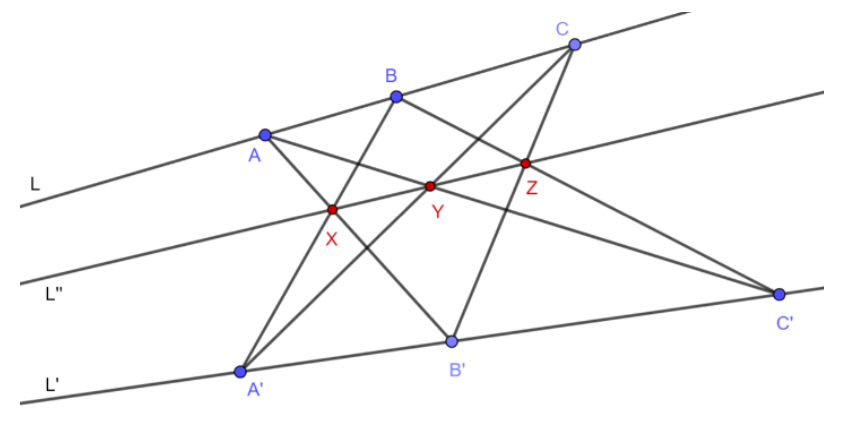
\includegraphics[width = 0.7\linewidth]{pappus.png}
        \end{center} 
        The points $X, Y, Z$ are always colinear. [Note: the diagram he drew in class had points labelled differently, I changed them because this diagram is from the internet. ]
    \end{theorem}
    \begin{proof}
        Take the line through $Y$ and $Z$, send it via a projective transformation to the line at infinity. Then, to show $X$ is on the same line as $Y, Z$ it suffices to show that after the transformation $\overline{AB'}$ is parallel to $\overline{A'B}$.\par 
        Suppose after the transformation the lines intersect at point $O$. 
        \begin{center}
            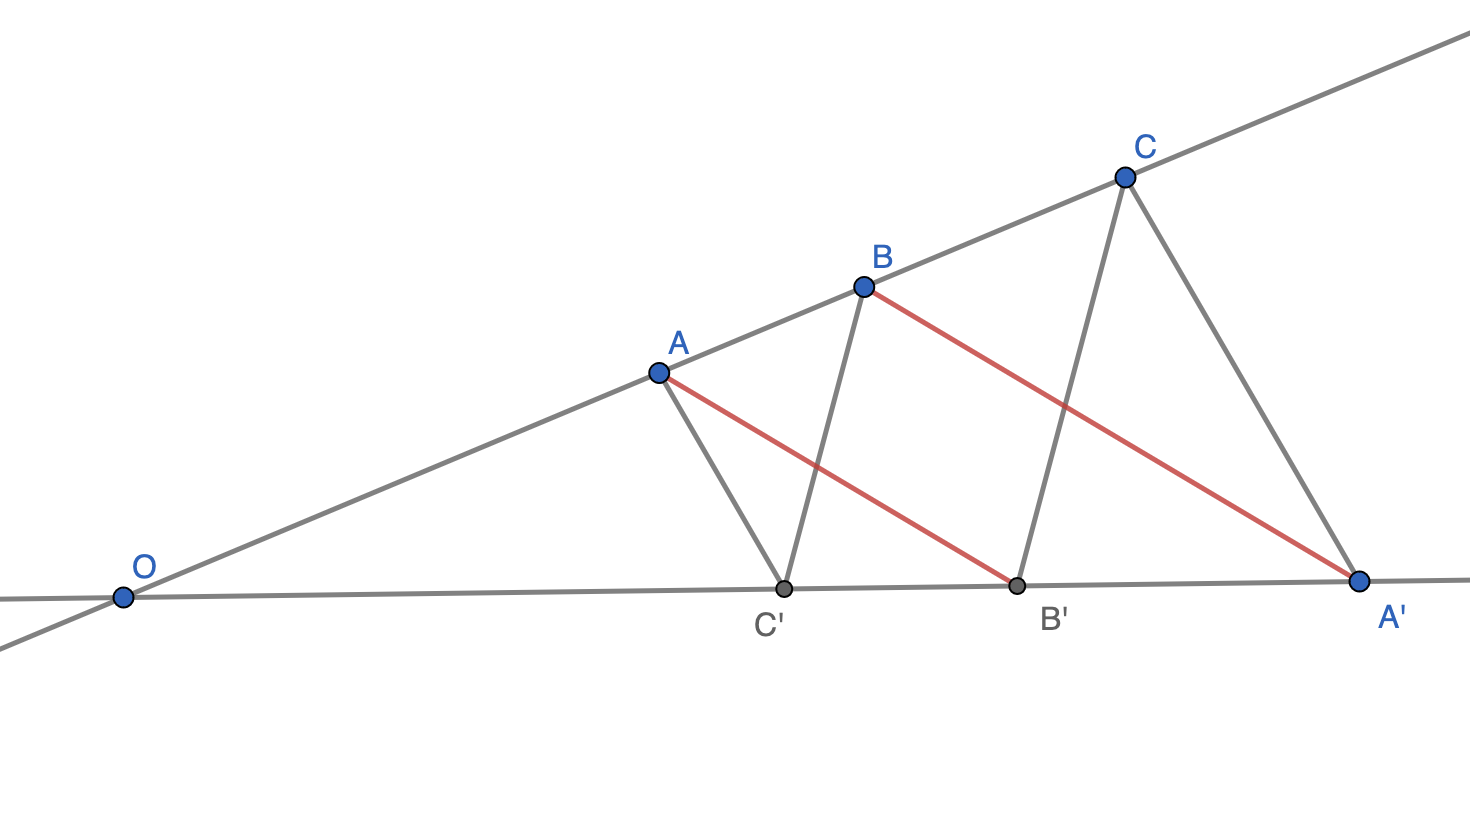
\includegraphics[width = 0.8\linewidth]{pappus_case_2.png}
        \end{center} 
        Because $AC'$ and $A'C$ are parallel, as well as $BC'$ and $B'C$, we have that $\triangle AOC'$ and $\triangle COA'$ are similar, same with $\triangle BOC'$ and $\triangle COB'$. From this we obtain the relations
        $$\frac{|OA|}{|OC'|} = \frac{|OC|}{|OA'|} \quad \frac{|OB|}{|OC'|} = \frac{|OC|}{|OB'|}$$
        Then, 
        $$\frac{|OA|}{|OB|} = \frac{|OA|}{|OC'|}\frac{|OC'|}{|OB|} = \frac{|OC|}{|OA'|}\frac{|OB'|}{|OC|} = \frac{|OB'|}{|OA'|}$$
        Because they share an angle and because a pair of their corresponding sides has the same ratio, triangles $\triangle AOB'$ and $\triangle BOA'$ must be similar. By the parallel line postulate we are done.
    \end{proof}

    For $\P^1$, recall that $\PGL_2(\F) = \{\frac{ax+b}{cx+d} \mid ad - bc \neq 0\}$. By the theorem above, elements of $\PGL_2(\F)$ send any three distinct points to any three distinct points. This is not true however for four points, so it makes sense that there would be some sort of invariant associated with four points. 
    \begin{definition}
        If $x_1, x_2, x_3, x_4 \in \P^1$ are distinct, \textbf{cross ratio} of these points is defined 
        $$[x_1, x_2, x_3, x_4] = \frac{(x_1-x_2)(x_3-x_4)}{(x_1-x_4)(x_3-x_2)}$$
        If $x_4 = \infty$, 
        $$[x_1, x_2, x_3, \infty] = \frac{x_1 - x_2}{x_3 - x_2}$$
        Similarly define for any other $x_i = \infty$. 
    \end{definition}
    \begin{theorem}
        If $f \in \PGL_2(\F)$ then $[f(x_1), f(x_2), f(x_3), f(x_4)] = [x_1, x_2, x_3, x_4]$. So, cross ratio is an invariant of $\PGL_2(\F)$.
    \end{theorem}
    \begin{proof}
        Note that $\PGL_2(\F)$ as a group is generated by the elementary matrices (considered as being projective transformations) of the form 
        $$\begin{pmatrix}
            a & 0 \\
            0 & d 
        \end{pmatrix} \quad 
        \begin{pmatrix}
            1 & b \\
            0 & 1
        \end{pmatrix} \quad 
        \begin{pmatrix}
            0 & 1 \\
            1 & 0
        \end{pmatrix}$$
        The first matrix acts on $x \in \P_\F^1$ by multiplying it by $a/d$. This of course does not change the cross ratio. The second matrix maps $x \mapsto x + b$, which also doesn't change the cross ratio, since $b$'s cancel in each pair of parentheses in the expression for the cross ratio. The last matrix maps $x \mapsto 1/x$. In this case, if $x_i < \infty$, 
        $$\frac{\left(\frac{1}{x_1} - \frac{1}{x_2}\right)\left(\frac{1}{x_3} - \frac{1}{x_4}\right)}{\left(\frac{1}{x_1} - \frac{1}{x_4}\right)\left(\frac{1}{x_3} - \frac{1}{x_2}\right)} = \frac{(x_2 - x_1)(x_4 - x_3)}{(x_4-x_1)(x_2-x_3)}$$
        Which is the same as the original cross-ratio. If say $x_4 = \infty$ we have 
        $$\frac{\left(\frac{1}{x_1} - \frac{1}{x_2}\right)\left(\frac{1}{x_3} - \frac{1}{x_4}\right)}{\left(\frac{1}{x_1} - \frac{1}{x_4}\right)\left(\frac{1}{x_3} - \frac{1}{x_2}\right)} = \frac{\left(\frac{1}{x_1} - \frac{1}{x_2}\right)\frac{1}{x_3}}{\left(\frac{1}{x_1}\right)\left(\frac{1}{x_3} - \frac{1}{x_2}\right)} = \frac{x_2 - x_1}{x_2 - x_3}$$
        which is again the same as the original cross ratio. Since all the generators of $\PGL_2(\F)$ preserve the cross ratio, so must all its elements. 
    \end{proof}
    Note that $[x_1, x_2, x_3, x_4] = [x_{\sigma(1)}, x_{\sigma(2)}, x_{\sigma(3)}, x_{\sigma(4)}]$ for $\sigma \in K$, the Klein $4$-group in $S_4$, so in fact $\sigma \in S_4$ can only change $[x_1, x_2, x_3, x_4]$ into $\lambda, 1-\lambda, 1/\lambda, 1-1/\lambda, \lambda/(\lambda-1), 1/(1-\lambda)$. Proving this will be an exercise. \par 
    \begin{proposition}
        Let $l_1, l_2 \in \P^2$, $O \in \P^2$ not on $l_1$ or $l_2$. Consider a projection of $l_1$ onto $l_2$ about $O$, as in the diagram (with $O$ unlabelled on top): 
        \begin{center}
            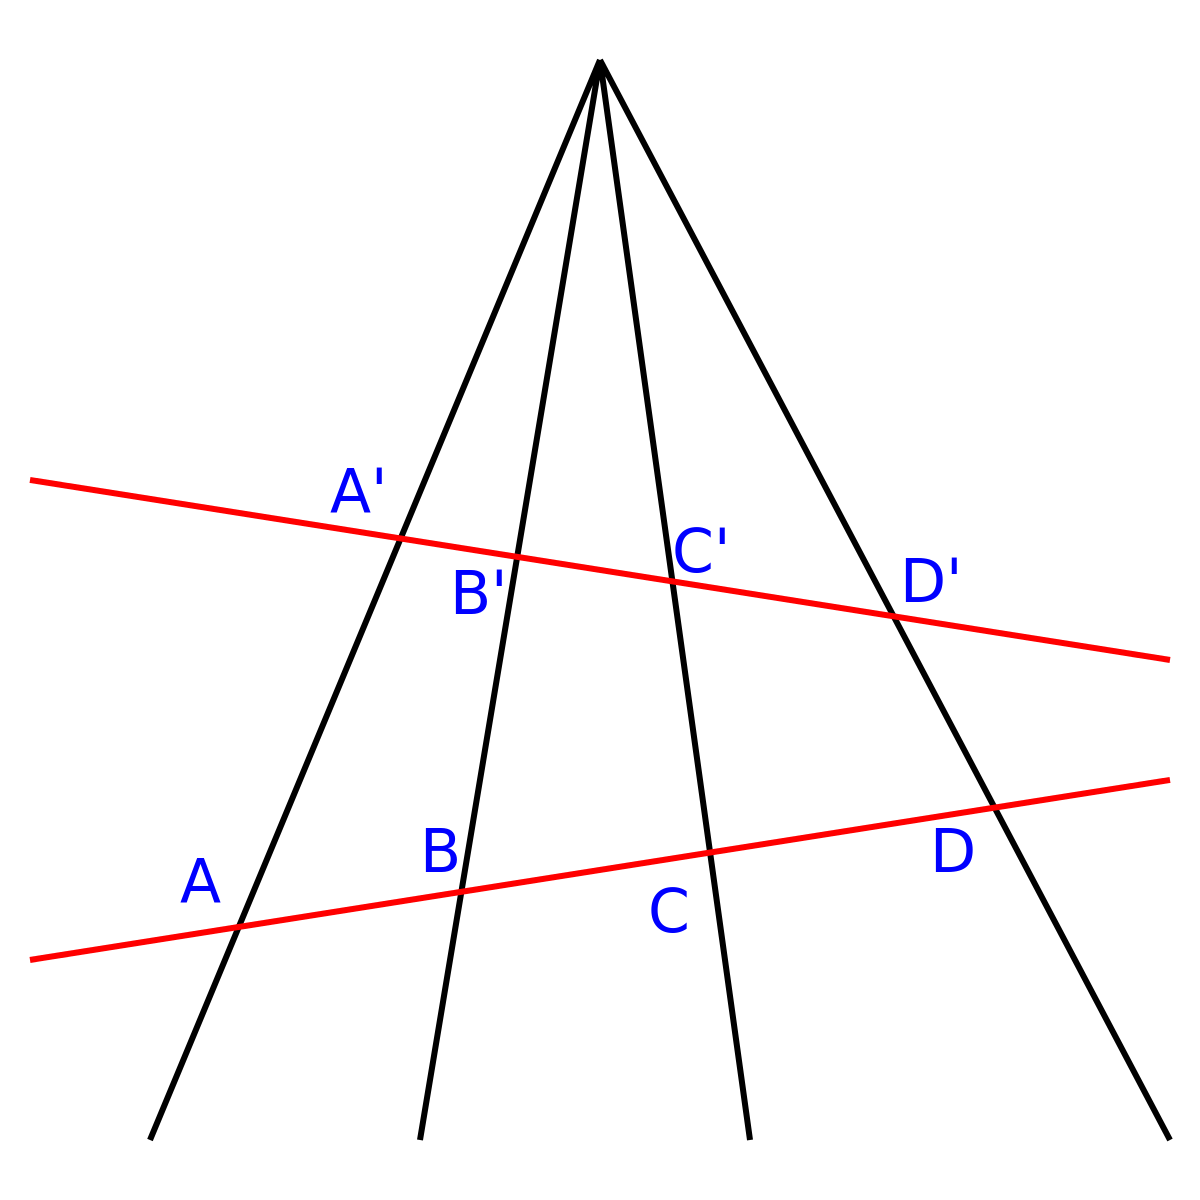
\includegraphics[width = 0.4\linewidth]{crossratio.png}
        \end{center}
        More precisely, if $A' \in l_1$ and $\vec{OA'}$ is a line in $\P^2$ containing both $O$ and $A'$, this map is $A' \mapsto A = \vec{OA'} \cap l_2$. This is a projective transformation. 
    \end{proposition} 
    Note that using this diagram, the invariance of cross ratio can be interpreted as the equivalence of ratios segments, as such: 
    $$\frac{|C'A'|}{|C'B'|}: \frac{|D'A'|}{|D'B'|} = \frac{|CA|}{|CB|}: \frac{|DA|}{|DB|}$$
    [A proof of this equality with elementary trigonometry is in Prasolov]
    \begin{proof}
        Let $L_1, L_2$ be planes and $O$ be a line in $V = \F^3$ not contained in either plane. Take the plane $V/O$, then $\P(V/O) = \P^1$. Then $L_i \to V \to V/O$, the composition of inclusion and quotient, gives us a map $\P^1 \to \P^1$. As a map between planes, this takes a point on $p \in L_i$ to its perpendicular projection onto $V/O \neq L_i$. This map is a bijective homomorphism, so its invertible. Indeed, we have the commutative diagram
        \[\begin{tikzcd}
            & V && V \\
            {L_1=\mathbb{P}^1} && {V/O=\mathbb{P}^1} && {L_2 = \mathbb{P}^1}
            \arrow[hook, from=2-1, to=1-2]
            \arrow[hook, from=2-5, to=1-4]
            \arrow[from=1-2, to=2-3]
            \arrow[from=1-4, to=2-3]
            \arrow[from=2-1, to=2-3]
            \arrow[from=2-5, to=2-3]
        \end{tikzcd}\]
        With the bottom two arrows being isomorphisms. Composing the left arrow with the inverse of the right arrow gives us a map in $\GL_2(\F)$ between $L_1$ and $L_2$, which induces the projection map in $\PGL_2(\F)$.  
    \end{proof}
    In particular, this implies that a projective transformation on $\P^2$ preserves cross ratio. 

    \subsection{Lecture 4} 
    Note we may write $R = \F[x_0, \dots, x_n] = R_1 \oplus R_2 \oplus \dots$ where $R_d$ is a vector space of homogeneous polynomials with degree of terms being $d$ (so $x_0^{k_0}x_1^{k_1} \dots x_n^{k_n}$ with $\sum k_i = d$). $R_0$ is the base field. $R_1$ is the dual space $V^*$ of $V = \F^n$ ($\{x_i\}$ is precisely the basis of $V^*$ dual to the standard basis $\{e_i\}$ of $V$). $R_2 = \mathbb{S}^2 V^*$, and in general $R_d = \mathbb{S}^d V^*$. 
    \begin{definition}
        Let $F \in R_d$ be a homog. polynomial with $d \neq 0$. Then the set of solutions of an equation $F(x_0, \dots, x_n) = 0$ is called a \textbf{hypersurface} of degree $d$ in $\P^n$.  
    \end{definition}
    \begin{example}
        In $\P^3$, $x_0^3 - x_1^3 + x_2x_3^2 + x_3^3 = 0$. The intersection of this with $\A^3$ (obtained by dividing all terms by $x_3$) is $(x_0/x_3)^3 - (x_1/x_3)^3 + x_2/x_3 + 1 = 0$. The rest of this hypersurface is in $\P^3 \setminus \A^3 = H$, in this $H$, the hypersurface is defined by $x_0^3 - x_1^3 = 0$. Since $H \cong \P^2$, we can do the same procedure to reduce this hypersurface to something we can draw in $\A^2$, getting $y_0^3 - y_1^3 = 0$, which are three lines intersecting at the origin (if $\F = \C$). Going the other way from $y_0^3 + y_1^3 + y_2 + 1 = 0$ by introducing another variable and going into $\P^3$ is called \textit{homogenization}. 
    \end{example}
    \begin{definition}
        A \textbf{projective variety} is a \textit{finite} intersection of hypersurfaces. 
    \end{definition}
    (Note: you do not get more sets if you extend this to an infinite system, by the Hilbert basis theorem, to be covered later). \par 
    \begin{definition}
        A hypersurface $X = \{F = 0\}$ for $F \in R_d$ is \textbf{irreducible} precisely when $F$ is irreducible. 
    \end{definition}
    \begin{example}
        \begin{itemize}
            \item $x_0x_1 = 0$ in $\P^2$ is a union of two lines. Not irreducible polynomial, so the hypersurface is not irreducible also. In general, any union of two lines is not irreducible. 
            \item $x_0^2 + x_1^2 = x_2^2$ is irreducible, so is its hypersurface, a circle in $\A^2$. 
        \end{itemize}
    \end{example}
    Assume $\F = \C$. Consider  the action of $\PGL_{n+1}$ on degree $d$ hypersurfaces in $\P^n$. Take $d = 1$, then this action is transitive, as we saw last time. Thus up to projective transformations all hyperplanes are the same. If $d = 2$, polynomial $F$ looks like 
    $$\sum a_{ij} x_i x_j = (x_0, \dots, x_n) A \begin{pmatrix}
        x_0 \\
        \vdots \\
        x_n
    \end{pmatrix} = x^\top A x$$
    With a symmetric matrix $A$. Subject to a projective transformation, $x = Uy$ for some $y \in \P^2$, $U \in \PGL_{n+1}$. Thus, $x^\top A x = 0 \mapsto (Uy)^\top A (Uy) = y^\top (U^\top A U) y^\top 0$. Note that because $A$ is symmetric, it is diagonalizable, hence for some $U$, $U^\top A U$ is a diagonal matrix of eigenvalues of $A$. In this case, we have shown:
    \begin{theorem}
        Any quadric is a projectively equivalent to a quadric $\lambda_0x_0^2 + \lambda_1x_1^2 + \dots + \lambda_nx_n^2 = 0$ (with some $\lambda_i$ possibly zero). 
    \end{theorem}
    If $\F = \R$, for $n = 2$ the picture is complicated, for example $x_0^2 - x_1^2 - x_2^2 = 0$ is a double cone. But for $\F = \C$ things become simpler because everything can be reduced to the cases $x_0^2 + x_1^2 + \dots + x_i^2 = 0$ (from the theorem above by applying a shearing transformation). So in $\P_\C^2$ we have lines, intersections of two lines, and conics, for $i = 1, 2, 3$ respectively. Thus the action of $\PGL_3$ has three orbits, namely those classes. \par 
    Now we discuss projective duality. Suppose we are working in $\P^2$. A line here is defined by an equation $ax + by + cz = 0$ with not all $a, b, c = 0$, modulo rescaling. Thus lines in $\P^2$ also form a projective space. This has some striking applications. \par
    Conceptually, if we have $\P^n = \P(V)$ for an $n$-dim vector space $V$, hyperplanes in $\P^n$ are in bijection with the elements of $\P(R_1) = \P(V^*)$. \par 
    The \textbf{duality principle} can be stated as follows. Consider any theorem about points and lines in $\P^2$, replacing `lines' by `points' and vice versa gives another valid theorem. 
    \begin{example}
        Recall Pappus' theorem. We can state it as follows: Consider lines $l_1, l_2$ and points $A, B, C$ on $l_1$ and $A', B', C'$ on $l_2$. Let $X$ be the intersection of lines $AB'$ and $A'B$, $Y$ the intersection of $AC'$ and $A'C$, and $Z$ the intersection of $BC'$ and $B'C$. Then $X, Y, Z$ are colinear. \par 
        The dual is: Given points $l_1, l_2$ and lines $A, B, C$ through $l_1$ and $A', B', C'$ through $l_2$, let $X$ be the line through points $AB'$ and $A'B$, intersections of lines $A \cap B'$ and $A' \cap B$ respectively. Define $Y, Z$ similarly. Then lines $X, Y, Z$ intersect in some point $O$. Diagram below: 
        \begin{center}
            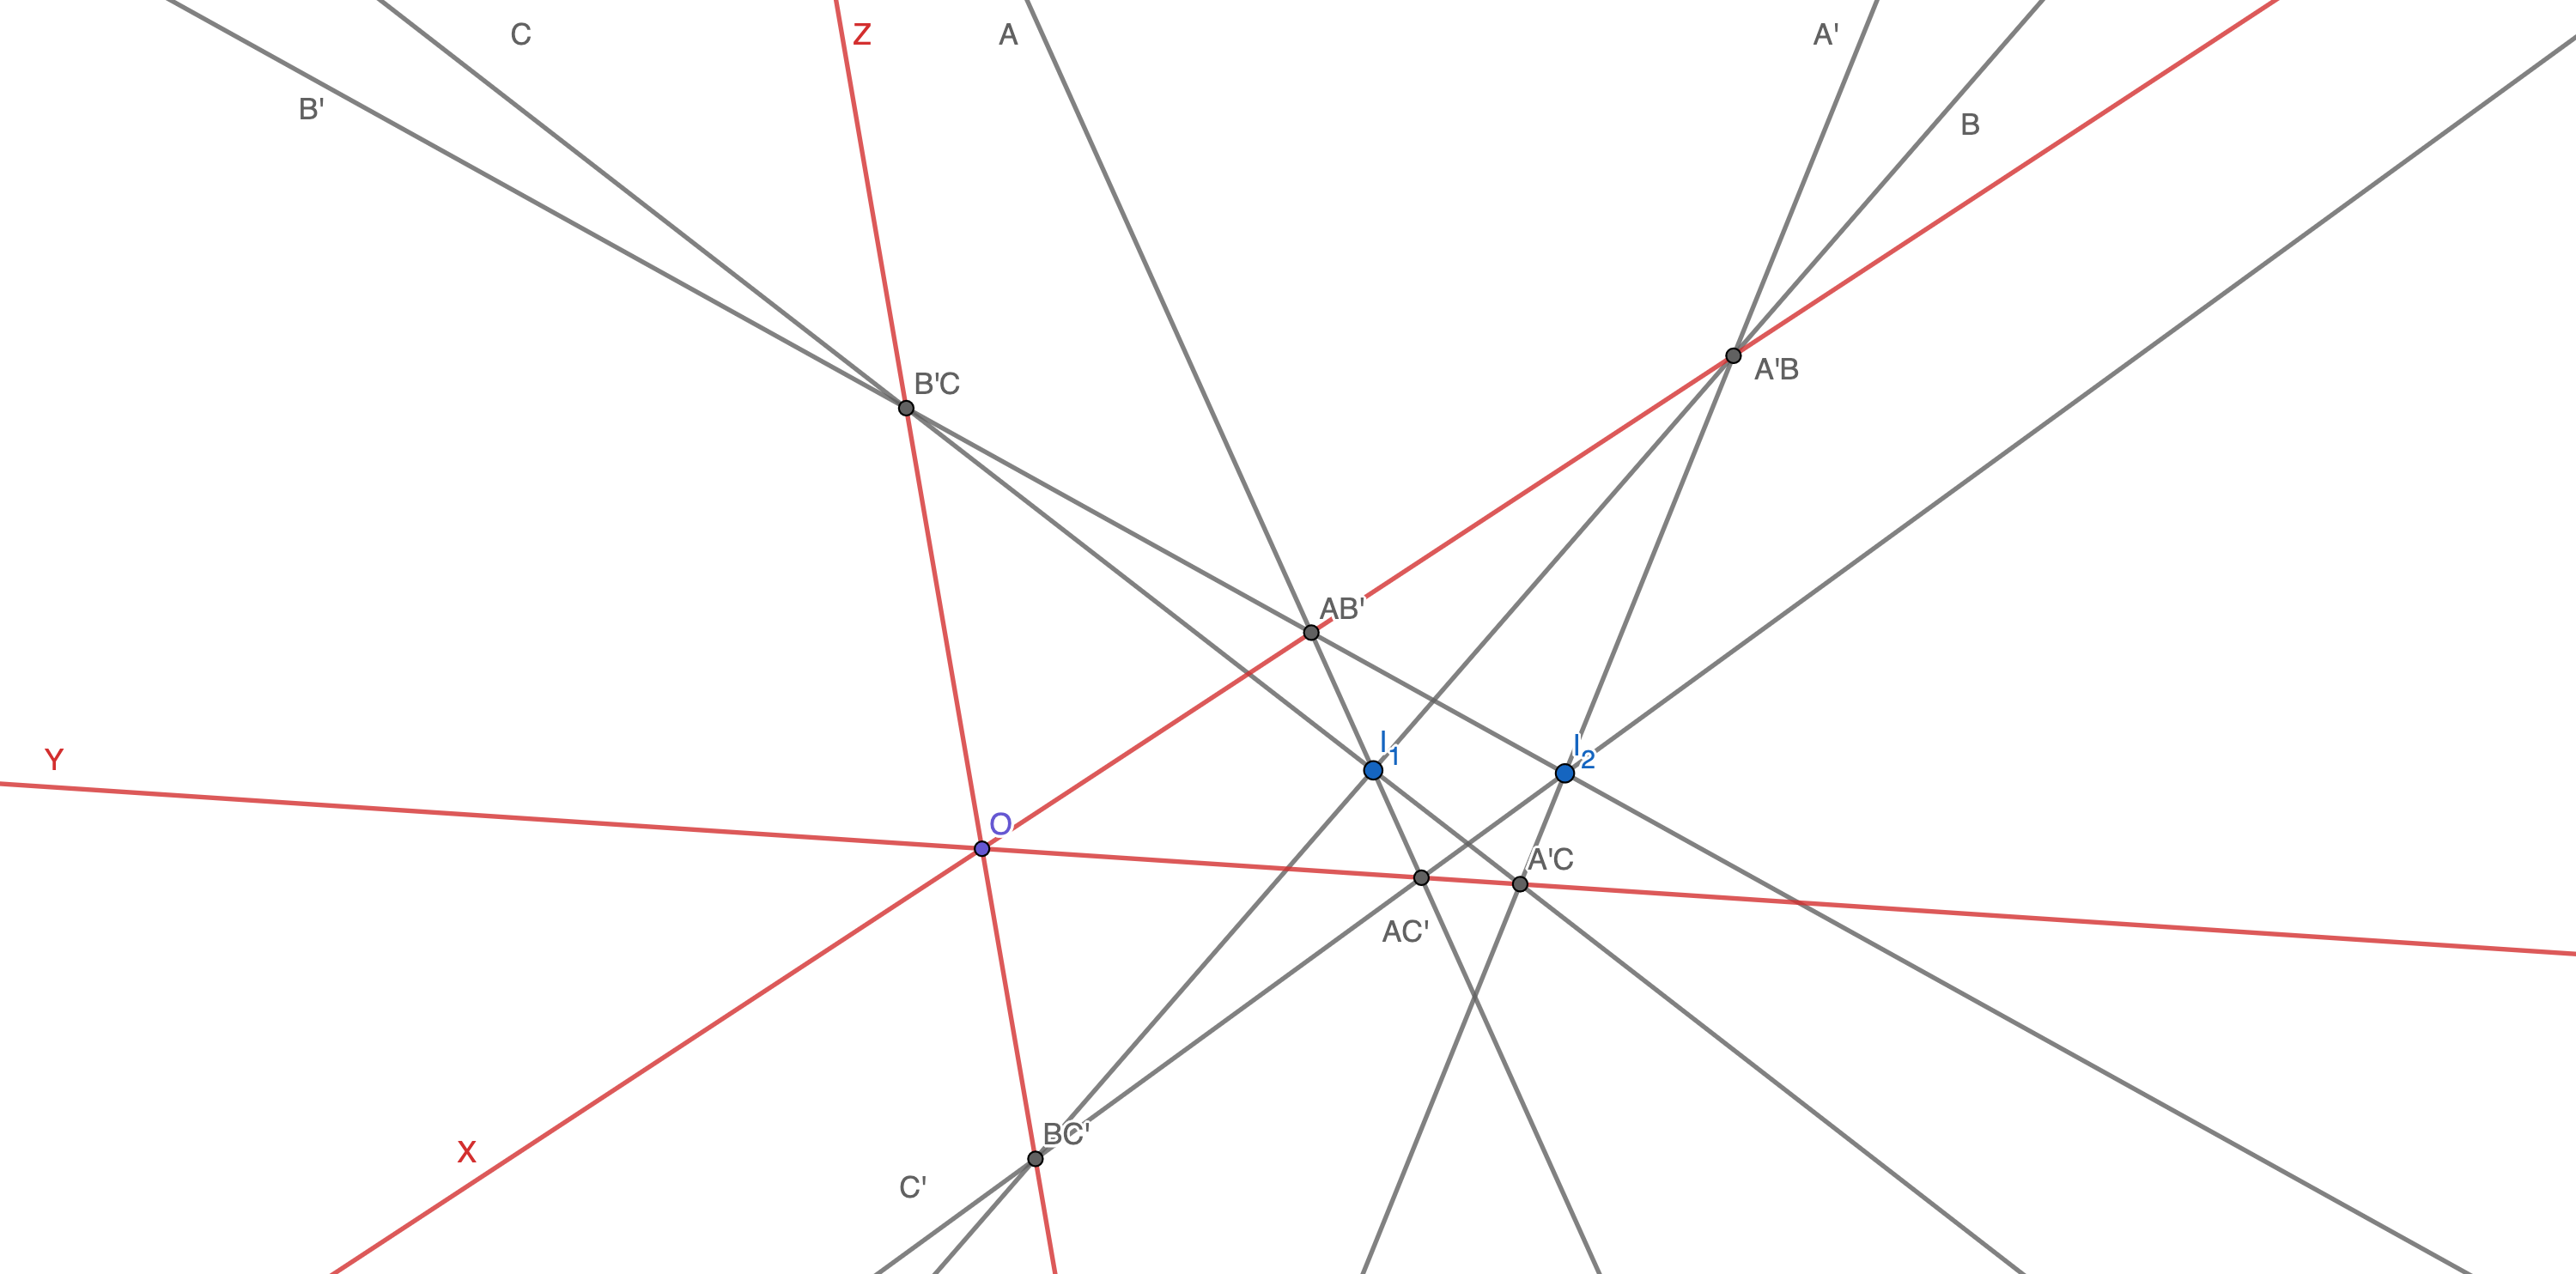
\includegraphics[width = \linewidth]{pappus_dual.png}
        \end{center}
    \end{example} 
    In $\P^3$ a similar duality holds: points correspond to planes, lines correspond to lines, planes correspond to points. \par 
    Three important facts about $V^*$: 1. $\dim V = \dim V^*$ since $V$ and $V^*$ are (not canonically) isomorphic, 2. $V \cong (V^*)^*$ canonically via an isomorphism $v \mapsto (\phi: V \to F \mapsto \phi(v))$, 3. There is an inclusion reversing bijection between subspaces of $V$ and $V^*$, which is equivalent to $\dim W + \dim W^\top = \dim V$. 

    \subsection{Lecture 5}
    Let's talk about conics a little bit more. If $\P_\F^n = \P(\F^{n+1})$, $[x_0: x_1: \dots : x_n]$ are homogeneous coordinates on $\P_\F^n$, and $P(x_0, \dots, x_n)$ is a homogeneous polynomial of degree $d$, we have that $\{[x_0, \dots, x_n] \mid P(x_0, \dots, x_{n+1}) = 0\} \subset \P^n$ is a hypersurface of degree $d$. For $d = 1$ this is the familiar hyperplane. If $d = 2$ this is a \textit{quadric}. \par 
    Over $\C$ (polynomials with coeffs in $\C$), every quadric is either a union of two lines, a cross of two lines, or a conic (which are all the same on the projective plane). A conic is called the \textit{smooth} quadric. \par 
    \begin{theorem}[Pascal]
        \hfill
        \begin{center}
            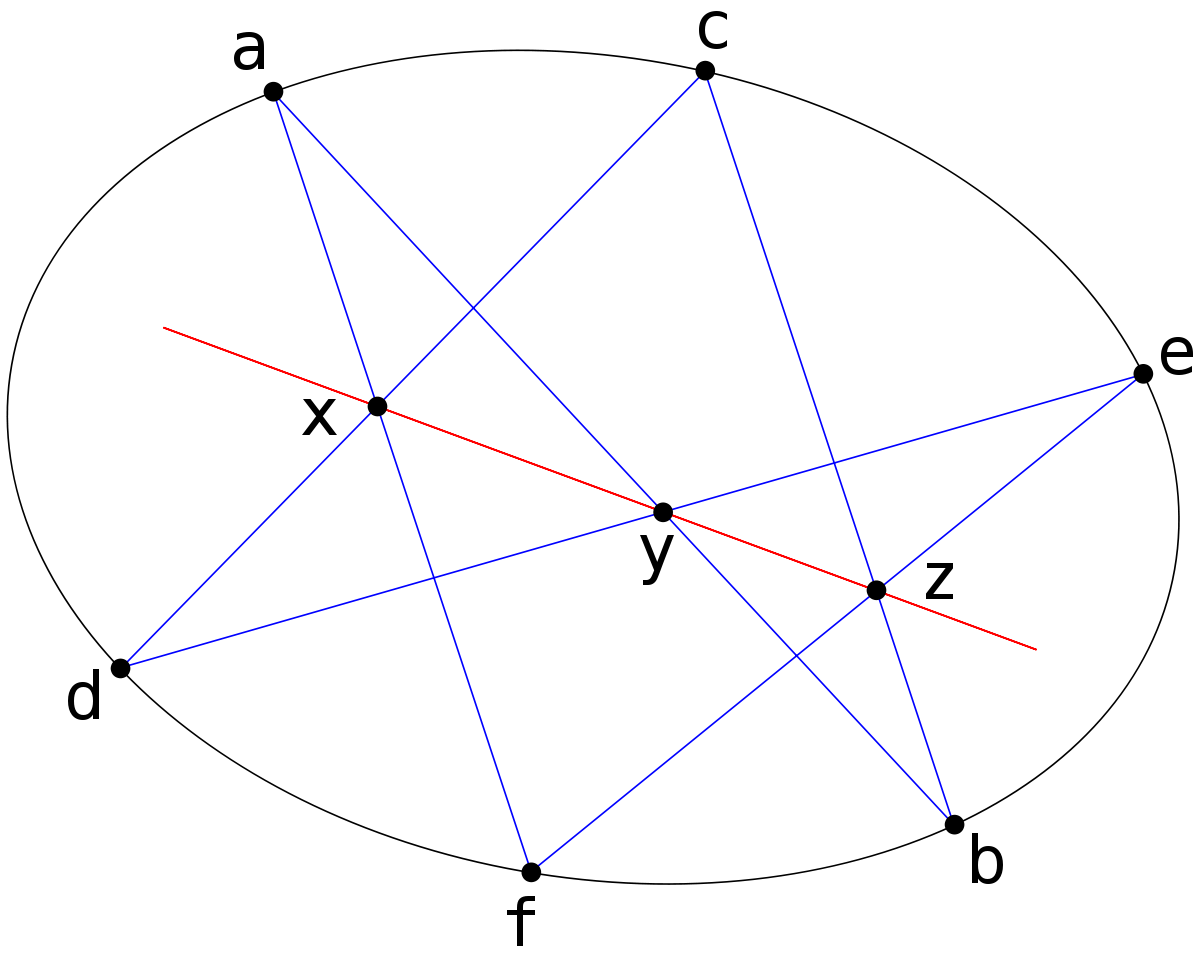
\includegraphics[width = 0.4\linewidth]{pascal.png}
        \end{center}
        For any ellipse, putting distinct $A, B, C, D, E, F$ on it and connecting them a la Pappus' theorem gives us colinear intersection points $X$, $Y$, $Z$. 
    \end{theorem}
    ``Who thinks this is beautiful? If you don't [points to door]''\par 
    In this way Pappus' theorem is not surprising because both a pair of lines and a conic are quadrics over $\C$. \par 
    \begin{lemma}[Chasles]
        Let points $A_1, A_2, A_3, A_4$ and $X$, $Y$ lie on a conic. Then 
        $$[(XA_1), (XA_2), (XA_3), (XA_4)] =  [(YA_1), (YA_2), (YA_3), (YA_4)]$$
        (Identification of a conic with $\P^1$ is explained below).
    \end{lemma}
    Notice that there is a bijection between points of a conic and lines through some particular point $X$ on a conic $C$. Indeed, a line through $X$ is either tangent to the conic or intersects it at some other point. Associating the tangent line to $X$ with infinity and the other lines to their intersection points, we associate the points of $C$ with $\P^1$. Indeed, the result above follows by using the two bijections onto $\P_1$ given by $X$ and $Y$, and concluding that there is a projective transformation mapping the $X$ configuration to the $Y$ configuration. This however requires some details we haven't gone over, so below is an elementary proof:
    \begin{proof}
        Without loss of generality assume the conic $C$ is a circle in $\R^2 \subset \P_\R^2$. If the points are ordered $A_1, \dots, A_4$ from left to right, let $U$ and $V$ be intersection points of a line $A_1A_4$ through $XA_2, XA_3$. (see diagram below)
        \begin{center}
            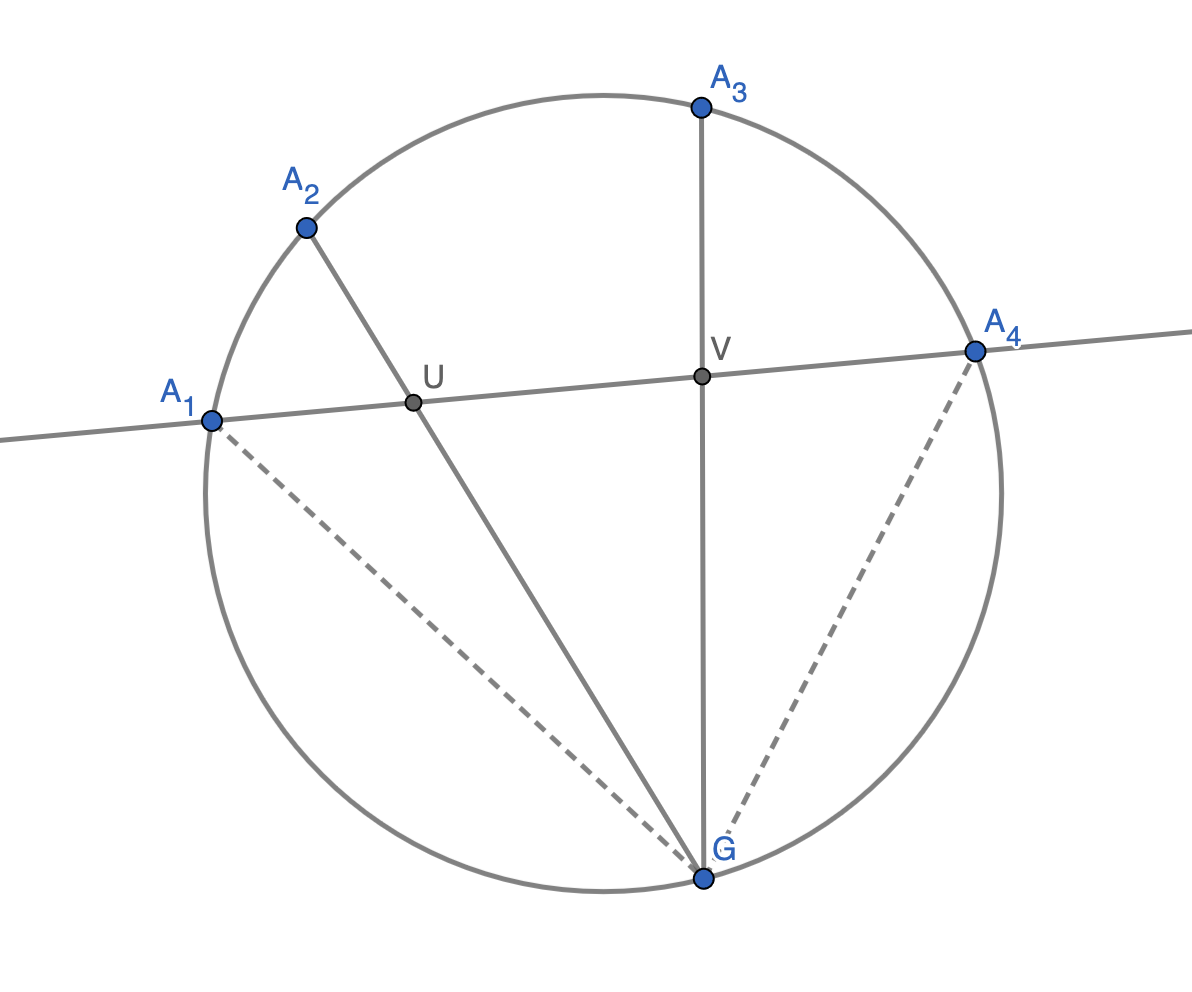
\includegraphics[width = 0.6\linewidth]{chasles.png}
        \end{center}
        Then
        $$[XA_1, \dots, XA_4] := [X_1, U, V, X_4] = \pm \frac{S_{A_1XY} S_{VXA_1}}{S_{A_1XA_2}S_{UXV}} = \frac{\sin \angle X_1XU \sin \angle VXA_1}{\sin \angle A_1XA_2 \sin \angle UXV}$$
        where $S_{ABC}$ is the notation for the area of triangle $ABC$ (we get the second equality since the altitude to $X$ is the same). Since they are inscribed angles, we know that they remain invariant if we replace $X$ with $Y$. We thus have shown that the cross ratio remains the same. 
    \end{proof}
    \begin{proof}
        [Proof: (Of Pascal's)] (TODO: relabel points either on diagram or here) By the lemma above, 
        $$[A_1B_1, A_1B_2, A_1B_3, A_1A_2] = [A_3B_1, A_3B_2, A_3B_3, A_3A_2]$$
        Now label the two intersection points above the line $XYZ$ in the diagram $S$ and $T$. Then by definition of cross ratio of four lines, 
        $$[B, Z, S, A_2] = [T, X, B_3, A_2]$$
        by picking the transversal line to be $A_2B_1$ and $A_2B_3$ for the left and right cross ratios respectively. But this quantity is also equal to $[(B_1Y), (ZY), (SY), (A_2Y)]$. We want $X$ and $Z$ to be colinear with $Y$, let $X'$ be the intersection of the line $ZY$ with $A_2B_3$. Then, 
        $$[(B_1Y), (ZY), (SY), (A_2Y)] = [T, X', B_3, A_2] = [T, X, B_3, A_2]$$
        This implies $X = X'$, which concludes the proof. 
    \end{proof}
    Our goal now is to go towards Bezout's theorem. The statement of the theorem is as follows: In $\P_\C^2$ let $X$ and $Y$ be projective curves such that they do not have common irreducible components. Then the number of points in their intersection is less than or equal to the product of their degrees, and in fact (hard part) is \textit{equal} to the product up to multiplicity. The hard part about the equality is that It's hard to define exactly what `up to multiplicity' means. Take two concentric circles $x^2 + y^2 = 1$ and $x^2 + y^2 = 2$ in $\A^2$. These only have solutions once you homogenize them and pass over to the complex projective plane. Then, $x^2 + y^2 = z^2, x^2 + y^2 + 2z^2$ have solutions $[1:i:0], [1:-i:0]$. By Bezout's these points have to have intersection multiplicty $2$, so in fact they are \textit{tangent points}. \par 
    For now, we will only prove the easier upper bound on the number of intersection points. 
    \begin{theorem}[Sylvester]
        Let $A(x) = a_mx^m + a_{m-1}x^{m-1} + \dots a_0 = 0$ and $B(x)$ be polynomials of degree $m$ and $n$ respectively. They have a common factor of degree $\geq 1$ if and only if the following $(m+n) \times (m+n)$ matrix
        $$\begin{bmatrix}
            a_m & a_{m-1} & \dots & a_0 & 0 & \dots & 0 \\
            0 & a_m & \dots & a_1 & a_0 & \dots & 0 \\
            & & \vdots & & \\
            0 & 0 & \dots & a_m & \dots & & a_0 \\
            b_n & b_{n-1} & \dots & &  b_0 & \dots & 0 \\
            0 & b_n & \dots & & & \dots & 0 \\
            & & \vdots & & \\
            0 & 0 & \dots & b_n & & \dots & & b_0 \\
        \end{bmatrix}$$
        (where $a_i$ appear in the first $n$ rows, $b_j$ appear in the last $m$ rows) has determinant $0$. The determinant is called the \textbf{resultant} of $A$ and $B$. 
    \end{theorem}
    \begin{proof}
        $A$ and $B$ have a common factor iff there exist non-zero polynomials $U$ and $V$ of degrees less than $n$ and $m$ respectively, such that $A\cdot U = B \cdot V$. This is a linear combination in the first $n$ rows being equal to a linear combination of the last $m$ rows, hence this condition holds iff $\det = 0$.  
    \end{proof}
    You can use this theorem to solve systems of polynomial equations by eliminating a variable, writing the condition that there is a solution in terms of the resultant. This is highly impractical if the degrees of equations are large, but is a useful proof technique. 

    \subsection{Lecture 6}
    Note that to generalize Sylvester's theorem to also work for polynomials over a ring and not a field we need to use Gauss' lemma. 
    \begin{theorem}
        Suppose that $f(x) = a_m(x-t_1)\dots (x-t_m)$, and $g(x) = b_n(x-s_1)\dots (x-s_n)$. Then their resultant is
        $$\Res(f, g) = a_m^n b_n^m \prod_{i=1}^m \prod_{j=1}^n (t_i - s_j)$$
    \end{theorem}
    \begin{proof}
        Let's view $\Res(f, g)$ as a polynomial in $\Z[a_m, b_n, t_1, \dots, t_m, s_1, \dots, s_n]$ (can do by Vieta's formulas). Looking at the resultant matrix, we can extract an $a_m$ and $b_n$ from every row of the determinant, we get $\Res = a_m^n b_n^m P(t_1, \dots, t_m, s_1, \dots, s_n)$. \par 
        Now we mention a little trick: for $f(x)$ with coefficients in a unique factorization domain, $f(x_0) = 0$ iff $(x-x_0)$ divides $f(x)$. Indeed, take $\tilde{f}(x) = f(x + x_0) = \tilde{a}_nx^n + \dots + \tilde{a}_0$. But then $f(x) = \tilde{a}_n(x-x_0)^n + \dots + \tilde{a}_0$, which $(x - x_0)$ divides if and only if $\tilde{a}_0 = 0$, i.e. $x_0$ is a root. \par 
        Thus, $P$ is divisible by $(t_i - s_j)$, since considering $P$ as a polynomial with coefficeints in $\Z[t_1, \dots, \hat{t}_i, \dots, t_m, s_1, \dots]$. Thus, $P(s_j) = 0$ implies $(t_i - s_j) \mid P$. Note that $(t_i - s_j)$ are pairwise coprime, as such 
        $$\Res(f, g) = Ca_m^n b_n^m \prod \prod (t_i - s_j)$$
        Note that the product $\prod \prod (t_i - s_j)$ has the same degree $nm$ as $\Res(f, g)$ (exercise), so by plugging in a point we realize $C = 1$. 
    \end{proof}
    (Discriminants, Resultants, and Multidimensional Determinants - very underrated book)\par 
    \begin{theorem}
        [Weak Bezout] Let $F$ be an infinite field, consider two curves with no common irreducible components in $\P_\F^2$, defined by $P(X, Y, Z) = 0$, $Q(X, Y, Z) = 0$ with $P$ and $Q$ homogeneous (no common irreducible components means $P$ and $Q$ are coprime). Then, $P$ and $Q$ have at most $\deg P \deg Q$ solutions. 
    \end{theorem}
    \begin{proof}
        Let $\deg P = m$, $\deg Q = n$. Assume the system $\{P = 0, Q = 0\}$ has $nm + 1$ solutions of the form $(X_i, Y_i, Z_i)$. Note there exists a coordinate system such that \textbf{1}. $P$ and $Q$ are not divisible by $Z$ and \textbf{2}. $Z_i \neq 0$ \textbf{3}. $\frac{Y_1}{Z_1}, \dots, \frac{Y_{n+m}}{Z_{n+m}}$. Then we have $f(x, y) = \frac{P(X, Y, Z)}{Z^m}$, $g(x, y) = \frac{Q(X, Y, Z)}{Z^n}$ are polynomials of degree $m$ and $n$ respectively in $X/Z$, $Y/Z$. They also have $nm + 1$ solutions $(x_i, y_i)$ with all $y_i$ distinct, and $f$ and $g$ have no common factor of degree $\geq 1$. Let's view $f(x, y), g(x, y)$ as polynomials in $(\F[y])[x]$. Note that $\Res(f, g)$, a polynomial in $\F[y]$, is nonzero with roots $y_i, \dots, y_{nm+1}$. It remains to show that $\deg \Res(f, g) < nm$. Left as a (non-trivial) exercise. 
    \end{proof}
    % An application of this theorem. Suppose we are working in $\P_\C^2 = \P(\C^3)$. Curves of degree $1$ are lines, they form $\P(V^*) = \P^2$ as we have seen before. Curves of degree $2$ of form $ax^2 + bxy + cy^2 + dxz + eyz + fz^2$ form a space $\P^5$ (dimension one less than the number of coordinates, since we can take $f = 1$). All degree $2$ curves containing a point $[x_0, y_0, z_0]$ form a ($4$-dimensional) hyperplane in $\P^5$. Space of degree $2$ curves containing $2$ points $P_1, P_2$ will have dimension at least $3$, but it can be $4$. Degree $2$ curves containing $P_1, P_2, P_3$ will have dimension at least $2$, ... we thus can show that any $5$ points in $\P^2$ lie on a unique quadric of degree $2$. 

    \subsection{Lecture 7}
    \begin{theorem}
        Let $P_1, \dots, P_5 \in \P^2$ be points in general position (no three points lie on the same line). Then there exists a unique conic containing $P_1, \dots, P_5$. 
    \end{theorem}
    \begin{proof}
        Consider $\P^5 = \P(\S^2V^*)$, the space of quadrics $F = ax^2 + by^2 + cz^2 + dxy + exz + yz$ in $\P^2$, corresponding to the coordinate $[a:b:c:d:e:1]$. For a $P \in \P^2$, the set $H_{P_i}$ of quadrics containing $P_i = [x_i:y_i:1]$ forms a $4$-hyperplane in $\P^5$, the intersection of $\P^5$ with a $5$-hyperplane in $\C^6$ corresponding to the set $ax_0^2 + by_0^2 + cz_0^2 + dx_0y_0 + ex_0z_0 + y_0z_0 = 0$. Because $P_i = [x_i: y_i: z_i] = [x_i/z_i: y_i/z_i: 1]$ are in general position, then so are vectors $[x_i^2, y_i^2, z_i^2, x_iy_i, x_iz_i, y_iz_i] = [(x_i/z_i)^2, (y_i/z_i)^2, 1, x_iy_i/z_i^2, x_i/z_i, y_i/z_i]$ (look at the last two coordinates). Hence, the $5$ hyperplanes corresponding to $H_{P_i}$ in $\C^6$ are in general position also, so they must intersect at precisely one point. Thus, $P_i$ specify a unique quadric. Because $P_i$ are in general position, we cannot have the quadric be a line or a union of two lines, because then one of the lines would have to contain three of the points. Hence, the quadric containing these points is indeed a conic. 
    \end{proof}
    Using this we can prove Pascal's theorem in a different way:
    \begin{theorem}
        [Pascal's theorem on conic] Take $C = 0$ defining an irreducible conic, $A_1, \dots, A_6$, $X = A_1A_5 \cap A_2A_6$, .... Then $X, Y, Z$ lie on the same line. 
        \begin{center}
            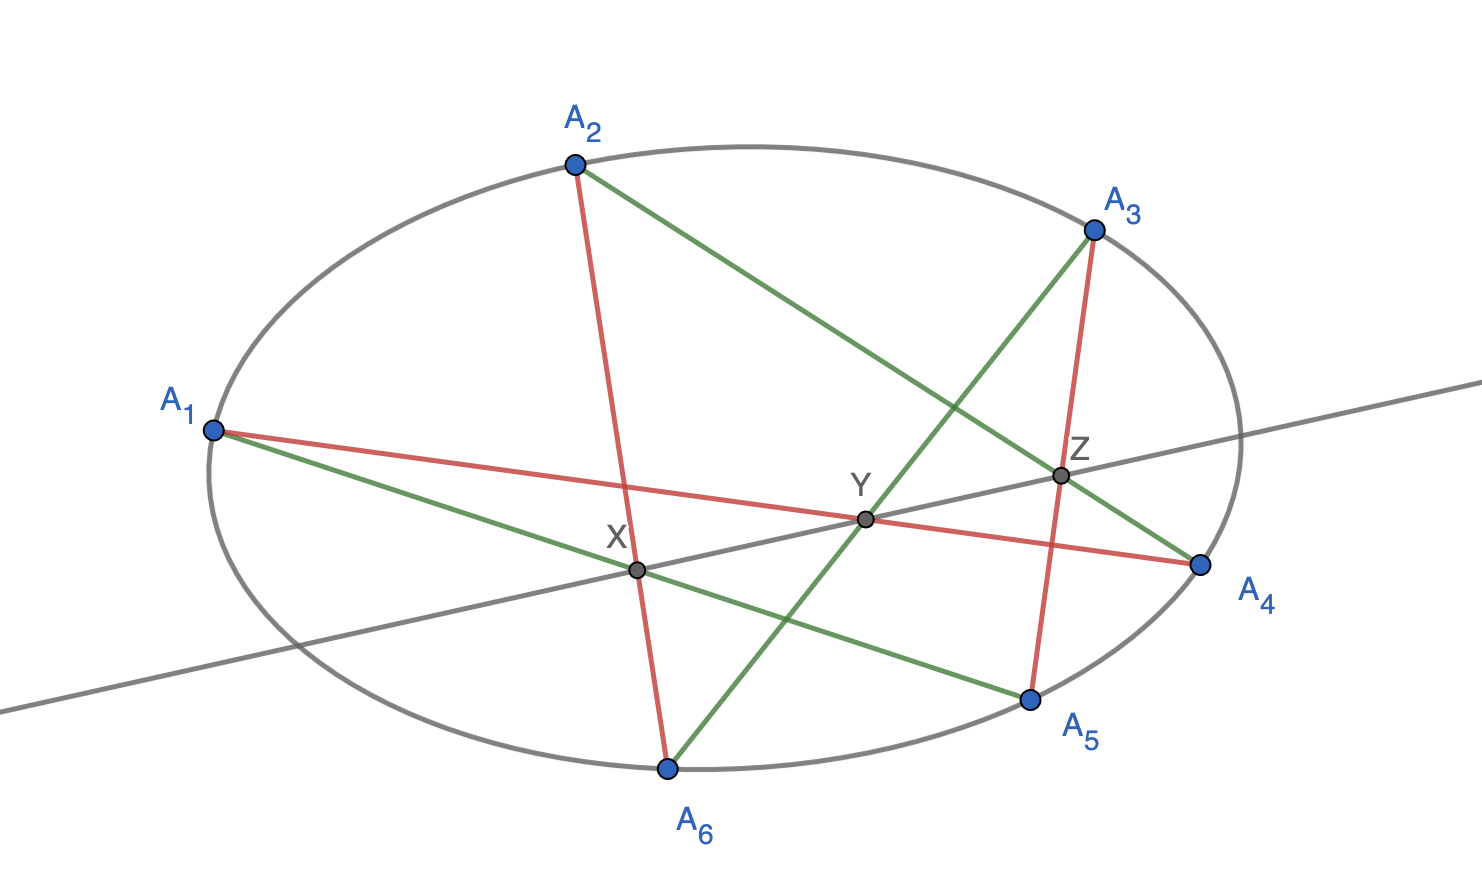
\includegraphics[width = 0.7\linewidth]{pascal_pf.png}
        \end{center}
    \end{theorem}
    \begin{proof}
        Denote by $L_{UV}$ be the equation for the line through some points $U, V$. Consider cubic curves $R = L_{A_6A_2}L_{A_5A_3}L_{A_1A_4}$ (in red) and $G = L_{A_1A_5}L_{A_2A_4}L_{A_3A_6}$ (in green). These intersect at $A_1, \dots, A_6, X, Y, Z$. Consider any point $P \in C$ that is not $A_1, \dots, A_6$. Then there exists $\lambda_p \in \C$ such that $(R + \lambda_p G)(P) = 0$ [Take $\lambda_p = \frac{-R(P)}{G(P)}$]. Then $R + \lambda_p G = 0$ is degree $3$ curve that has $7$ points in common with the quadric $C$. But by weak Bezout's, $C$ and $R + \lambda_p G$ can intersect in at most $6$ unless they have a component in common. Since $C$ is irreducible, their common component must be $C$ itself, hence $R + \lambda_p G$ must be a union of $C$ and a line. The three points $X$, $Y$, $Z$ that do not lie on $C$ must then lie on a line. 
    \end{proof}

\section{Algebraic Geometry}
    For $\A^n$, $R = k[x_1, \dots, x_n]$, and an ideal $I \subset R$ we have a \textbf{vanishing ideal} $V(I) = \{(a_1, \dots, a_n) \in \A^n \mid f(a_1, \dots, a_n) = 0 \text{ for any } f \in I\}$. For finitely generated $I = (f_1,\dots, f_n) = \{g_1f_1 + \dots + g_nf_n\}$, we have that $V(I)$ is the set of solutions of $\{f_i(x_1, \dots, x_n) = 0\}$. We will prove soon that all ideals of $k[x_1, \dots, x_n]$ are finitely generated. People call $V(I)$ \textbf{affine sets}, affine algebraic sets, affine algebraic varieties, or affine closed sets. \par 
    Some properties: 
    \begin{enumerate}
        \item $V((1)) = \emptyset$.
        \item $V((0)) = \A^n_k$.
        \item For ideals $I, J \subset k[x_1, \dots, x_n]$, 
        $$V(I) \cup V(J) = V(IJ)$$
        where $IJ$ is the ideal generated by products $fg$ for $f \in I$, $g \in J$. 
        \begin{proof}
            Inclusion $V(I) \cap V(J) \subset V(IJ)$ is obvious. For the other inclusion, if $p \not \in V(I)$ then for any $f \in I$, $f(p) \neq 0$. Similarly $p \not \in V(J)$ implies any $g \in V(J)$ doesn't vanish on $p$. So if $p \not \in V(I) \cup V(J)$, $fg(p) \neq 0$ also, hence $p$ cannot be in $V(IJ)$.
        \end{proof}
        \item For a collection of ideals $I_\alpha \subset k[x_1, \dots, x_n]$, 
        $$\cap_\alpha V(I_\alpha) = V(\sum_\alpha I_\alpha)$$
        where $\sum_\alpha I_\alpha$ is an ideal consisting of sums of elements in various $I_\alpha$, i.e. one generated by the elements of $\cup I_\alpha$.
        \begin{proof}
            If $p \in \cap_\alpha V(I_\alpha)$, then polynomials in every $I_\alpha$ vanish on $p$, hence their sums vanish also. If $p \in V(\sum_\alpha I_\alpha)$, for any $\alpha$ any element of $I_\alpha$ vanishes on $p$, hence the other inclusion holds.  
        \end{proof}
    \end{enumerate}
    These properties imply that affine sets are closed sets of a topology on $\A^n_\F$, called the \textbf{Zariski topology}. \par 
    ``I have 20 more minutes? *Claps hands*''\par 
    \begin{example}
        \begin{enumerate}
            \item If $\A_\C^1$, $R = \C[x]$, thus affine algebraic sets are either finite collections of points or $\A^1$.
            \item In $\A^2_\C$ we have a more complicated picture, we could have finite collections of points + quadrics and lines. 
        \end{enumerate}
    \end{example}

    \begin{definition}
        Suppose $R$ is a ring (commutative with $1$). $R$ is \textbf{Noetherian} if (TFAE)
        \begin{enumerate}
            \item Every ideal $I \subset R$ is finitely generated. 
            \item Every ascending chain $I_1 \subset I_2 \subset I_3 \subset \dots \subset R$ stabilizes, so for some $N$, $I_{N} = I_{N+1} = I_{N+2} = \dots$. 
        \end{enumerate} 
    \end{definition}
    Equivalence of these two conditions is on HW3. Geometrically, the Noetherian condition will tell us that infinite systems don't give us any new options for affine sets. \par 
    \begin{example}
        \begin{enumerate}
            \item A field $\F$, every ideal is generated by $0$ or $1$. 
            \item $\Z$, $\F[x]$, generated by $a \in \Z$ and $x^n$ respectively. 
            \item If $R$ is Noetherian, $R/I$ is Noetherian. 
            \item Hilbert basis theorem: If $R$ is Noetherian, $R[x]$ is Noetherian. 
            \item $F[x_1, \dots, x_n]$ is Noetherian. 
            \item By the above $F[x_1, \dots, x_n]/I$ is Noetherian. In particular, we will study $\C[x, y]/(x^2 + y^2 + 1)$, vanishing functions on a circle. 
        \end{enumerate}
    \end{example}
    (Vakil Spectral theory notes are very good)\par 
    \begin{theorem}
        [Hilbert Basis Theorem] $R$ Noetherian if and only if $R[x]$ is Noetherian. 
    \end{theorem}
    \begin{proof}
        One direction is simple: if $I$ is an ideal of $R$, it is also an ideal of $R[x]$. If $R[x]$ is Noetherian, $R$ is finitely generated as an ideal of $R[x]$, but since $I$ is also an ideal of $R$, all its generators must be in $R$ also. But then $I$ is finitely generated over $R$ also. \par 
        In the other direction, say $I \subset R[x]$ is an ideal, and let $f_0$ be an element in $I$ of the smallest degree, $f_1$ be an element of smallest degree in $I - (f_0)$, $f_2$ smallest degree in $I - (f_0, f_1)$ ...($-$ is set subtraction). Suppose for contradiction that $I$ is not finitely generated, so we can keep choosing $f_i$ indefinitely. Consider the leading coefficients $a_i$ of $f_i$, and the chain of ideals 
        $$(a_0) \subseteq (a_0, a_1) \subseteq (a_0, a_1, a_2) \subseteq \dots$$
        This is an ascending chain of ideals in $R$, hence it must stabilize at some ideal $(a_0, \dots, a_{n-1})$. Thus, the ideal of leading coefficients of $f_i$ must be generated by $a_1, \dots, a_{n-1}$. In particular, the leading coefficient $a_{n}$ of $f_{n}$ can be expressed like $\lambda_1 a_1 + \dots + \lambda_{n-1} a_{n-1}$.
        Then consider
        $$g = f_{n} - (\lambda_1 f_1 x^{\deg f_{n} - \deg f_1} + \dots + \lambda_{n-1} f_{n-1} x^{\deg f_{n} - \deg f_{n-1}})$$
        (Note that by construction of our $f_i$, the exponents are valid) The leading term in the parentheses is the same as the leading term of $f_{n}$, so $\deg g < \deg f_{n}$. But also $g \in I - (f_1, \dots, f_{n-1})$ (since the term in the parantheses is in $(f_1, \dots, f_{n-1})$). This contradicts our choice of $f_n$ earlier, so we are done. 
    \end{proof}

    \subsection{Lecture 8}
    There exists a correspondence between ideals on $k[x_1, \dots, x_n]$ and affine algebraic sets in $\A^n$. Indeed, we can take any ideal $I$ on $k[x_1, \dots, x_n]$ and consider its vanishing set $V(I)$. 
    % Note the following properties we reviewed last time: $V(I \cap J) = V(I) \cup V(J)$ and $I \subset J \implies V(I) \supset V(J)$. 
    In the other direction, take some affine algebraic $X$ and consider $I(X) = \{f \in k[x_1, \dots, x_n] \mid \forall p \in X, f(p) = 0\}$. 
    So given $X$, we can relate to it the ideal of functions that vanish on it. Note however that this correspondence is not invertible: consider $I \subset \R[x, y]$ generated by $x^2 + y^2 + 1 = 0$. The vanishing set of this is empty, but $I(\emptyset) = \R[x, y]$ (also could consider $k = \C$ and first consider $I = (x^2)$). However:
    \begin{proposition}
        For any affine algebraic set $X \subset \A^n$ we have $V(I(X)) = X$. So, $X \to I(X)$ is an injective map.
    \end{proposition}
    \begin{proof}
        Set $X = V(f_1, \dots, f_n)$, so $X$ consists of points on which $f_i$ vanish. If $p \in X$, then $p \in V(I(X))$ obviously. On the other hand if $p \in V(I(X))$, then all $f \in I(X)$ vanish on $p$. In particular, $f_1, \dots, f_n \in I(X)$ vanish on $p$, hence $p \in X$. 
    \end{proof}
    \begin{definition}
        Let $I \subset R$ be an ideal in a ring. The \textbf{radical} of $I$, denoted $\sqrt{I}$, is given by $\{z \in \R \mid \exists N\: z^N \in I\}$. 
    \end{definition}
    This is an ideal (homework). An example of how this works is $\sqrt{(x^2)} = (x)$. 
    \begin{definition}
        $I$ is \textbf{radical} if $\sqrt{I} = I$. 
    \end{definition}
    \begin{theorem}
        [Hilbert's Nullstellensatz] For an ideal $J \subset k[x_1, \dots, x_n]$ ($k$ is algebraically closed), we have $I(V(J)) = \sqrt{J}$.  
    \end{theorem}
    Example: $(x^2) \xrightarrow{V} 0 \in \A^1 \xrightarrow{I} (x) = \sqrt{(x^2)}$. \par 
    `Middle school version': consider $f_1, \dots, f_m \in \C[x_1, \dots, x_n]$. Suppose that $g \in \C[x_1, \dots, x_n]$ vanishes at every solution of the system $\{f_i = 0\}_i$. Then there exists some positive integer $N$ such that $g^N$ is in $(f_1, \dots, f_n)$, an ideal of $\C[x_1, \dots, x_n]$. \par 
    \begin{definition}
        An affine algebraic set $X$ is called \textbf{irreducible} if it cannot be presented as a union of affine algebraic sets. Thus, if $X = X_1 \cup X_2$ is irreducible, $X_1$ or $X_2$ is $X$. 
    \end{definition}
    \begin{theorem} \label{thm:irr_iff_prime}
        $X$ is irreducible iff $I(X)$ is prime. 
    \end{theorem}
    \begin{proof}
        Suppose $I(X)$ is not prime, so there exist $f, g \in k[x_1, \dots, x_n]$ with $fg \in I(X)$ but $f$ or $g \not \in I(X)$. Take $X_1 = X \cap V(f)$, $X_2 = X \cap V(g)$. Then $X = X_1 \cup X_2$, but $X_1, X_2 \neq X$ since otherwise $f$ or $g \in I(X)$. \par 
        Suppose $X$ is not irreducible, so $X = X_1 \cup X_2$ with $X_1, X_2 \neq X$. So $I(X) \neq I(X_1)$, in fact $I(X) \subset I(X_1)$, similarly $I(X) \subset I(X_2)$ (subsets strict). As such, there exist $f \in I(X_1) - I(X_2)$, $g \in I(X_2) - I(X_1)$, thus $fg$ vanishes on $X_1 \cup X_2$, so $fg \in I(X)$ but neither $f, g \in I(X)$. 
    \end{proof}
    \begin{theorem}
        Suppose $X \subset \A^n$ is an affine algebraic set. Then
        \begin{enumerate}
            \item There exist irreducible affine sets $X_1, \dots, X_m$ such that $X = X_1 \cup \dots \cup X_m$, and $X_i \not \subset X_j$ for any $i \neq j$. 
            \item This decomposition is unique up to relabeling the sets $X_i$. 
        \end{enumerate} 
    \end{theorem}
    \begin{proof}
        If $X$ is irreducible, we are done. Otherwise, $X = X_1 \cup X_2$, a union of proper algebraic subsets. Then decompose $X_1, X_2$, and continue recursively until we obtain a binary tree of affine sets, where the leaves (terminating nodes) are irreducible. Suppose for contradiction the tree we obtain this way is infinite, then there exists an infinite path down the tree: $X \supset X^{(1)} \supset X^{(2)} \supset \dots $. which corresponds to an infinite chain of ideals $I(X) \subset I(X^{(1)}) \subset I(X^{(2)}) \subset \dots $ with strict inclusions. But this contradicts the fact that $X$ is Noetherian. So the tree must be finite, which must give us a finite decomposition of $X$ into a union of irreducible sets $X_i$. To get the condition $X_i \not \subset X_j$, discard any set $X_i$ which violates it. \par 
        Suppose we have two decompositions $X_1 \cup \dots \cup X_m = X_1' \cup \dots X_m'$. Take any $X_i$, then $X_i = X \cap X_i = (X_1' \cap X_i) \cup (X_2' \cap X_i) \dots \cup (X_m' \cap X_i)$. Because $X_i$ is irreducible, we have $X_i = X_i \cap X_j'$ for some $j$, and as such $X_i \subset X_j'$. But performing this same argument for $X_j'$ we get $X_j' \subset X_k$, so $X_i = X_k$, and indeed $X_i = X'_j$. 
    \end{proof}
    Main example of affine sets are hypersurfaces: if $f(x_1, \dots, x_n)$ is an irreducible polynomial of non-zero degree, its vanishing set is an irreducible \textbf{hypersurface}. An example would be something like $xyz \pm x^2 + y^2 + z^2 + 1 = 0$. \par 
    Recall our correspondence between algebraic sets and ideals of $k[x_1, \dots, x_n]$ from the beginning. Note that by Nullstellensatz, $I(X)$ for any affine algebraic set $X$ is a radical ideal. So, restricting our correspondence to radical ideals, the correspondence becomes bijective. This same correspondence carries irreducible sets to prime ideals, hypersurfaces to principal ideals (as we've shown in Theorem \ref{thm:irr_iff_prime}), and maximal ideals to single points (this is shown in the next lecture). \par 
    % Now we need some notions from commutative algebra. Suppose $A$ and $B$ are algebras over the same field $k$. We say that $A$ is \textbf{finitely generated over $B$} if there exist $a_1, \dots, a_n \in A$ such that $A = B[a_1, \dots, a_n]$: every $a \in A$ is a polynomial in $a_1, \dots, a_n$ with coefficients in $B$. Example: $k[x_1,\dots, x_n]$ finitely generated algebra over $k$. Another one is $\C[x, y]/(x^2 + y^2 - 1)$, a finitely generated algebra over $\C$. \par 
    % We say $A$ is \textbf{finite} over $B$ [if $A$ is a finitely generated $B$-module] if there exist $a_1, \dots, a_n \in A$ such that for all $a \in A$ there are $b_1, \dots, b_n \in B$ so $a = a_1b_1 + \dots + a_n b_n$. In other words, $A = a_1B + a_2B + \dots + a_nB$. Example: $\C[x]/(x^3 - 1)$, this is a finite algebra over $\C$, in fact a three-dimensional vector space. If your algebra is also a field, another algebra being finite over it means you have a finite-dimensional vector space.  

    \subsection{Lecture 9}
    \begin{definition}
        An algebra $A$ over $k$ is \textbf{finitely generated over $B$} (another $k$-algebra) (sometimes denoted by the tower $A - B$) if there exist $a_1, \dots, a_n \in A$ such that every element in $A$ is a polynomial in $a_i$ with $B$-coefficients: $A = B[a_1, \dots, a_n]$.  
    \end{definition}
    In other words, $B[x_1, \dots, x_n] \to A$ with the map being the evaluation homomorphism $f \mapsto f(a_1, \dots, a_n)$ is surjective. By the first isomorphism theorem, $A \cong B[x_1, \dots, x_n]/I$.
    \begin{definition}
        $A$ is a \textbf{finite $B$-algebra} if there exist $a_1, \dots, a_n$ if for every $a \in A$ there exist $b_1, \dots, b_n$ such that $a = b_1a_1 + \dots + b_na_n$. In other words, $A = Ba_1 + \dots + Ba_n$. 
    \end{definition}
    Here's a key bit from commutative algebra, to be proven later:
    \begin{theorem} \label{thm:fin_if_fin_alg}
        Let $k$ be a field of characteristic $0$. Suppose that $A$ is a finitely generated over $k$. Assume $A$ is a field. Then $A$ is a finite $k$-algebra. 
    \end{theorem}
    (Choosing e.g. $k = \C$, we know that every finitely generated algebra over $\C$ that's a field must be $\C$ itself. )\par
    \begin{proposition}
        For $P = \{a = (a_1, \dots, a_n)\} \subset \A^n_k$, $I(P) \subset k[x_1, \dots, x_n]$ is maximal. Conversely, if $M \subset k[x_1, \dots, x_n]$ is maximal, then $V(M) \subset \A^n_k$ is a single point.
    \end{proposition}
    \begin{proof}
        Firstly, we show that $I(P)$ is precisely $(x_1 - a_1, \dots, x_n - a_n)$. The ideal $(x_1 - a_1, \dots, x_n - a_n)$ is clearly a subset of $I(P)$. On the other hand, take any $f \in I(P)$, then $f(a_1, \dots, a_n) = 0$, and $f(y_1 + a_1, \dots, y_n + a_n)$ is some polynomial in $y_i$ with coefficients in $k$. Plugging in $y = x_i - a_i$ we get that $f(x_1, \dots, x_n)$ is a polynomial in $x_i - a_i$ with coefficients in $k$, i.e. $f \in (x_1-a_1, \dots, x_n-a_n)$. We further claim $I(P) = (x_1 - a_1, \dots, x_n - a_n)$ is maximal. Consider the surjective map $k[x_1, \dots, k_n] \to k $ given by the evaluation homomorphism $f \mapsto f(a_1, \dots, a_n)$. Its kernel is $I(P)$. Then by the first isomorphism theorem, $k[x_1, \dots, x_n]/(x_1- a_1, \dots, x_n - a_n) \cong k$, a field, which implies $I(P)$ is maximal. \par 
        Conversely we show that for every maximal ideal $M \subset k[x_1, \dots, x_n]$ there exist $a_1, \dots, a_n$ such that $M = (x_1 - a_1, \dots, x_n - a_n)$. Indeed, consider $k[x_1, \dots, x_n]/M$, a finitely generated algebra over $k$ and a field, so by Theorem \ref{thm:fin_if_fin_alg} it is generated by some $b_1, \dots, b_n$ over $k$. Thus, the composition $\phi: k \to k[x_1, \dots, x_n] \xrightarrow{\pi} K = k[x_1, \dots, x_n]/M$ is such that there exist $a_i \in k$ with $\phi(a_i) = \pi(x_i)$. This implies that $(x_1 - a_1, \dots, x_n - a_n) \subset m$, but $(x_1 - a_1, \dots, x_n - a_n)$ as a maximal ideal, as proven above. Hence, $m = (x_1 - a_1, \dots, x_n - a_n)$. 
    \end{proof}

    Now we show 
    \begin{proposition}[Weak Nullstellensatz]
        The vanishing set of $k[x_1, \dots, x_n]$ is the empty set. In other words, if $J \subset k[x_1, \dots, x_n]$ is a proper ideal, $V(J) \neq \emptyset$. 
    \end{proposition}
    \begin{proof}
        Let $J = (f_1, \dots, f_n) \subset k[x_1, \dots, x_n]$, and suppose for the sake of contradiction that $V(J) = \emptyset$. Then there exists a maximal ideal $M = (x_1 - a_1, \dots, x_n - a_n)$ for some $a_i$ such that $(f_1, \dots, f_m) \subset (x_1-a_1, \dots, x_n - a_n)$. But $V(M) = \{P\}$ is non-empty, and $V(M) \subset V(J)$. Contradiction. 
    \end{proof} 

    Now we prove Nullstellensatz. 
    \begin{proof}
        % Suppose that $g \in k[x_1, \dots, x_n]$ vanishes at every point $p$ that's a solution to $\{f_i(p) = 0\}$ (this system has solutions). Then there exists $N$ such that $g^N \in (f_1, \dots, f_m)$. Consider $k[x_1, \dots, x_n] \subset k[x_1, \dots, x_n, t]$. Consider an ideal $J = (f_1(x_1, \dots, x_n), \dots, f_m(x_1, \dots, x_m), tg(x_1, \dots, x_m) - 1)$, we know $V(J) = \emptyset$. Then there exist some polynomials $u_1, \dots, u_{m+1} \in k[x_1, \dots, x_m, t]$ such that $u_1f_1 + \dots + u_mf_m + u_{m+1}(tg-1) = 1$. Plug in $t = \frac{1}{g}$, then $u_1(x_1, \dots, x_n, 1/g)f_1(x_1, \dots, x_n) + \dots = 1$, and 
        % $$\frac{\tilde{u}(x_1, \dots, x_n)}{g^m}f_1(x_1, \dots, x_m) + \dots + \frac{\tilde{u}(x_1, \dots, x_m)}{g^m} = 1$$
        % Multiply by $g^m$ on both sides and we are done. This type of reduction of strong to weak Nullstellensatz is called the Rabinovich trick.
        We show that for any $f \in J = (f_1, \dots, f_n)$, we have some $N$ such that $f^N \in J$. Consider the ideal $J_f \subset k[x_1, \dots, x_n, t]$ generated by $f_1, \dots, f_n, ft - 1$. Then its vanishing ideal $V(J_f) = \{(P, b) \in \A^{n+1}_k \mid P \in J(F), bf(P) = 1\}$ is empty as the conditions are contradictory. Hence, $J_f = k[x_1, \dots, x_n, t]$, in particular 
        $$1 = \left(\sum g_if_i\right) + g_{0}(ft - 1)$$
        Let $N$ be the degree of the right hand side as a polynomial in $t$. Then, consider 
        $$f^N = \left(\sum G_if_i \right) + G_0(ft - 1)$$
        where $G_i$ are polynomials in $x_1, \dots, x_n, ft$ (by construction there should be enough $f$ factors to associate each $t$ factor with an $f$ factor). Then, by passing this identity through the quotient by the ideal $(ft - 1)$ we get 
        $$f^N \equiv \sum h_i f_i$$
        where $h_i(x_1, \dots, x_n) = G_i(x_1, \dots, x_n, 1)$. But the quotient map is injective, hence this identity holds in $k[x_1, \dots, x_n]$. We conclude $f^N \in J$, so $I(V(J)) \subset \sqrt{J}$. Since the other inclusion is obvious, we are done.   
    \end{proof}
    Now we should probably prove the commutative algebra result we've been relying on. 
    \begin{lemma}
        If $A - B$ and $B - C$ are finite then $A - C$ is finite. 
    \end{lemma}
    \begin{proof}
        Express $A = a_1B + a_2B + \dots a_nB$, $B = b_1C + \dots b_mC$, plug in the latter into the former. 
    \end{proof}
    \begin{lemma}
        Suppose $A - B$ finite, then for $a \in A$ there exist $n \in \mathbb{N}$, $b_0, \dots, b_{n-1} \in B$ then $a^n + b_{n-1}a^{n-1} + \dots + b_0 = 0$ [$a$ is integral over $B$].
    \end{lemma}
    \begin{proof}
        $A$ is finite over $B$, thus there exist $a_1, \dots, a_n$ such that $A = Ba_1 + \dots + Ba_n$, so 
        $$\begin{cases}
            aa_1 = b_{11}a_1 + \dots + b_{1n}a_n \\
            aa_2 = b_{21}a_1 + \dots + b_{2n}a_n \\
            \vdots 
            aa_n = b_{n1}a_1 + \dots + b_{nn}a_n
        \end{cases}
        $$
        Subtracting $aa_i$ from the left we get a system, and from it we get 
        $$\det \begin{bmatrix}
            b_{11}-a & b_{12} & \dots & b_{1n} \\
            b_{21} & b_{22}-a & \dots & b_{2n} \\
            \vdots \\
            b_{n1} & b_{n2} & \dots & b_{nn}-a \\
        \end{bmatrix} = 0$$
        There exists an \textit{adjunct} matrix $X^*$ to the matrix $X$ above such that $X^*X = \det X \Id X^*$. Then we also get 
        $(\det X)a_i = 0$ and $\det X = b_1a_1 + \dots $ (TODO) 
    \end{proof}
    Final lemma:
    \begin{lemma}
         $B[x] - B$ is finite.
    \end{lemma}

    \subsection{Lecture 10}
    Now we should prove Theorem \ref{thm:fin_if_fin_alg} from above, because everything relies on it. Let's restate it: 
    \begin{theorem*}
        Let $k$ be an infinite field, and $A$ is a finitely generated algebra over $k$. Then $A$ is a finite algebraic extension of $k$. 
    \end{theorem*}
    We introduced three lemmas last time. Let's do a forth:
    \begin{lemma}
        Let $A$ be finite over $B$, If $A$ is a field, then $B$ is a field. 
    \end{lemma}
    \begin{proof}
        Suppose $b \neq 0 \in B$. Then, $\frac{1}{b} \in A$, consider 
        $$\frac{1}{b}^n + a_{n-1}\frac{1}{b}^{n-1} + \dots + a_0 = 0$$
        multiplying both sides by $b^n$, and factoring, we get that $1/b$ is in $B$. 
    \end{proof}
    \begin{theorem}
        [Noether Normalization Theorem] Let $A$ be a finitely generated algebra over $k$, so $A = k[a_1, \dots, a_n]$. Then there exist $y_1, \dots, y_m \in A$ such that 1. $y_1, \dots, y_m$ are algebraically independent and 2. $A$ is finite over $k[y_1, \dots, y_m]$. 
    \end{theorem}
    \begin{example}
        Take $\C[x, y]/(y^2 - x^3y - 1)$. Consider that $y$ is a root of a monic polynomial with coefficients in $\C[x]$ in this field, namely $y^2 - x^3y - 1 = 0$. Hence this field is finite over $\C[x]$. However, the same does not hold for $x$, so this field is not finite over $\C[y]$. Geometrically, the finiteness condition means that every time we get the same number of points on $y^2 - x^3y - 1$ for any fixed $x$ (up to multiplicity). This is not true for a fixed $y$. 
    \end{example}
    We can now show the commutative algebra result using Noether normalization. By it there exist $y_1, \dots, y_m$ such that $A$ is finite over $k[y_1, \dots, y_m]$. Thus, by lemma 4, $k[y_1, \dots, y_m]$ is a field, which can only be the case if $m = 0$, so $A$ is finite as an algebra over $k$. Thus, every element in $A$ is algebraic over $k$. \par 
    ``The elephant is not a field, unless it's not an elephant... You like the elephant? Everybody likes elephants, have you seen an elephant?'' \par 
    To prove Noether Normalization we need yet another lemma:
    \begin{lemma}
        Take $f \neq 0 \in k[x_1, \dots, x_n]$, $\deg f = d$. There exists a change of variable
         $$x'_1 = x_1 - \alpha_1 x_n, \dots, x'_{n-1} = x_{n-1} - \alpha_{n-1}x_n, x_n' = x_n$$
        such that $f(x_1' + \alpha_1x_n, \dots, x_{n-1}'+\alpha_{n-1}x_n, x_n)$ has a term $cx^d_n$ with $c \neq 0$.  
    \end{lemma}
    \begin{proof}
        Write $f = f_0 + f_1 + \dots + f_d$ where $f_i$ is a homogeneous degree $i$ polynomial. Then, $f_d$ is non-zero, so there exist $\alpha_i$ such that $f_d(\alpha_1, \dots, \alpha_{n-1}, 1)$, the coefficient of $x^d_n$, is non-zero.  
    \end{proof}
    \begin{proof}
        [Proof (Of Noether Normalization):] By induction, $A[a_1, \dots, a_n]$ finitely generated. Consider $k[x_1, \dots, x_n] \xrightarrow{\phi} A$ be a surjective homomorphism. If $I = \ker \phi = 0$ we are done. If $I \neq 0$, consider $f \neq 0 \in I$. Base case $n=1$: $A = k[a]$, $f(a) = 0$ implies $a$ is integral over $k$. Thus $k[a] - k$ is finite. Assume for $n-1$ this is known, take $k[a_1, \dots, a_n]$. Choose $\alpha_1, \dots, \alpha_{n-1}$ so $f(x_1' + \alpha_1x_n, \dots, x_{n-1}'+\alpha_{n-1}x_n, x_n)$ has a non-zero $x_n^d$ term, so $a_1' = a_1 - \alpha_1a_n$, ..., $a_{n-1}' = a_{n-1} - \alpha_{n-1}a_n$. As such, 
        $$\frac{1}{c}f(a_1' + \alpha_1a_n, \dots, a_n) = 0$$
        Hence $a_n$ is a root of a monic polynomial with coefficient in $k[a'_1, \dots, a'_{n-1}]$. Hence, $k[a_1, \dots, a_n] - k[a_1', \dots, a_{n-1}']$ is finite, using the inductive assumption, but now we can find $k[y_1, \dots, y_m]$ such that $k[a_1, \dots, a_n] - k[y_1, \dots, y_m]$ is finite. 
    \end{proof}
    \begin{definition}
        If $X$ is an afffine algebraic set $\subset \A^n$, a function $f: X \to k$ is called \textbf{regular} or ``polynomial'' if there exists $F \in k[x_1, \dots, x_n]$ such that for all $a = (a_1, \dots, a_n) \in X$ we have $f(a_1, \dots, a_n) = F(a_1, \dots, a_n)$. 
    \end{definition}
    \begin{example}
        Consider $X \subset \A^2$, $X = V(y-x^2)$. Then we have $f(x, y) = x^3 + y$ which ``equals'' $xy + y$ on $X$. 
    \end{example}
    Regular functions on $X$ form a $k$-algebra, taking $k[X]$ to be the coordinate ring of $X$, $k[x_1, \dots, x_n] \to k[X]$ has kernel $I(X)$. So coordinate ring of $X$ is $k[x_1, \dots, x_n]/I(X)$. 
    \begin{example}
        $k[\A^n] = k[x_1, \dots, x_n]$. Then functions on the circle $\C[x, y]/(x^2 + y^2 - 1)$ which ``equals'' $\C[\sin t, \cos t] = \C[e^{it}, e^{-it}]$, so should be true that $\C[u, v]/(uv - 1)$. This is indeed true, and nothing more than the statement that every circle and hyperbola are isomorphic over the complex numbers. 
    \end{example}
    Facts: 
    \begin{enumerate}
        \item $k[x] = k[x_1, \dots, x_n]/I(X)$ such that $I = \sqrt{I}$. So in the quotient there are no nilpotents $a^m = 0$ or $a \neq 0$. Thus this algebra is reduced. 
        \item $X$ is irreducible if and only if $I(X)$ is prime if and only if $k[x]$ is a domain. 
        \item $X$ is a point if and only if $I(X)$ is maximal iff $k[X] = k$. 
    \end{enumerate}

    \subsection{Lecture 11}
    Today we wil talk about the category of affine algebraic varieties and its equivalence to the category of reduced finitely generated $k$-algebras. \par 
    Reminder: a category is a set of objects, and morphisms between them. So for any two objects $X, Y$ there is a set of morphisms $\Mor(X, Y)$. Note that in $\Mor(X, X)$ there is a designated element called the identity $\id_X$. Also, there exists a composition operation $\circ: \Mor(X, Y) \times \Mor(Y, Z) \to \Mor(X, Z)$ that is associative and respects identity, so $(f \circ g) \circ h = f \circ(g \circ h)$ and $f \circ \id_X = \id_Y \circ f = f$. \par
    As an example, for any group you can take the elements of the group $g$ as morphisms from the same object, and define composition $g \circ h = gh$ using group multiplication. The identity element $e$ acts as the identity morphism on the object. \par
    Now, take $k$ to be an algebraically closed field. Take a category in which affine algebraic varieties $X = V(I) \subset \A^n$ with $I$ an ideal of $k[x_1,\dots, x_n]$ for some $n$ are the objects. Take the morphisms $f: X \to Y$ of these affine algebraic varieties, called either \textbf{regular maps} or \textbf{polynomial maps}, to be such that there exist $P_1, \dots P_m \subset k[x_1, \dots, x_n]$ so that for any $(b_1, \dots, b_n) \in X$, $f(X) = (P_1(b_1, \dots, b_n), \dots, P_m(b_1, \dots, b_n))$. One example of a regular map is something like $x \mapsto (x^3 + 1, x^2)$ between $X = \A^1 \to Y = \A^2$. ANother one is $(x_1, x_2) \mapsto x_1$. Taking $X$ to be the parabola $y = x^2$, the morphism $(x, y) \mapsto x$ maps $X$ to $Y$ being the $x$-axis. \par 
    In this category, the identity morphism is given by $(x_1, \dots, x_n) \mapsto (x_1, \dots, x_n)$. A composition of regular maps is again a regular map. \par 
    In any category there's a notion of an isomorphism, namely $f \in \Mor(X, Y)$ is an isomorphism if there exists a $g \in \Mor(Y, X)$ such that $f \circ g = \id_Y$ and $g \circ f = \id_X$. For example, the morphism $(x, y) \mapsto x$ from a parabola to the $x$-axis is an isomorphism, since $g$ from the axis to the parabola given by $x \mapsto (x, x^2)$ is its `inverse'. \par 
    Here is a conjecture, which ``will certainly give you a professor position here if you solve it''. Take isomorphisms $\A^n \to \A^n$ in the category of affine algebraic sets. For instance, take $(x, y) \mapsto (x^2 + y, x)$, its inverse is $(x, y) \mapsto (y, x-y^2)$. Notice that the determinant of the Jacobian of an isomoprhism is a non-zero constant, the converse, that it suffices for a regular map to have a non-zero constant Jacobian in order for it to be invertible, is called the Jacobian conjecture. \par 
    Let $X\subset \A^n$ be an affine algebraic variety, then $k[X] = k[x_1, \dots, x_n]/I(X) = \Mor(X, \A^n)$. Note that $k[X]$ is a finitely generated algebra over $k$, and $k[X]$ is \textbf{reduced}, i.e. has no nilpotent elements, which happens iff $I(X) = \sqrt{I(X)}$. \par 
    Consider now the category of reduced finitely generated algebras over $k$. Morphisms $\Mor(B, A)$ in this category being homomorphisms of $k$-algebras $B \to A$. Some examples:
    \begin{enumerate}
        \item $\C[x] \to \C$ via $x \mapsto 3$.
        \item $\C[y] \to \C[x, y]/(y^2 - x)$ via inclusion. 
        \item $\C[x, y]/(x^2+y^2-1) \xrightarrow{} \C[t_1, t_2]/(t_1t_2 - 1)$ so this is an isomorphism in the category.
    \end{enumerate} 
    We want to say that these categories are in some way the same. For this, define a map $F: \mathcal{C} \to \mathcal{D}$ between categories, called a \textbf{functor}. For any object $X \in \mathcal{C}$, a functor $F$ gives an object $F(X) \in \mathcal{D}$. For any morphism $f: X \to Y$ we have a map $F(f): F(X) \to F(Y)$. \par 
    Let a (contravariant) functor between the category of affine algebraic varities and finitely generated algebras over $k$ be given by $k[X] = k[x_1, \dots, x_n]/I(X)$. This functor takes a map $f: X \to Y$ given by $(x_1, \dots, x_n) \mapsto (F_1(x_1, \dots, x_n), \dots, F_m(x_1, \dots, x_n))$ to the map $k[Y] = k[y_1, \dots, y_m]/I(X) \to k[X] = k[x_1, \dots, x_n]/I(X)$ by $y_i \to F_i(x_1, \dots, x_n)$. \par 
    Some examples: 
    \begin{enumerate}
        \item The example of isomorphism between parabola and the $x$-axis corresponds to the map $\C[x] \to \C[x, y]/(y-x^2)$. 
        \item A map $\A^1 \to \A^2$ given by $x \mapsto (x, 3x-1)$ corresponds to $\C[x, y] \to \C[x]$ by $x \mapsto x$, $y \mapsto 3x-1$. 
    \end{enumerate}
    The most straightforward way to think of how to say that these two categories are equivalent is to come up with another functor $G$ such that $F \circ G = \id_\mathcal{C}$, $G \circ F = \id_\mathcal{D}$. However this almost never makes sense, the map in the other direction will involve choices and not be well-defined. The correct notion is the equivalence of categories. So, a functor $F$ gives an equivalence if there exists a natural transformation $F \circ G \to \id$, and in the other direction also. (We won't talk about what that means, watch Bouchard's category theory videos). Instead we will prove some facts about $F$ that should make it clear that it defines an equivalence. \par 
    \begin{proposition}
        $F$ is \textbf{essentially surjective}: For every finitely generated algebra $A$ there exists an affine algebraic variety $X$ s.t. $k[X] \cong A$, finitely generated implies $A \cong k[x_1, \dots, x_n]/I = k[X]$, $A$ is reduced implies for $V(I) = X\subset \A^n$, $I = \sqrt{I}$. (TODO)
    \end{proposition}
    \begin{proposition}
        $F$ is \textbf{fully faithful}: the map $\Mor(X, Y) \to \Hom(k[Y], k[X])$ given by $f \mapsto f^*$ given by $F$ is a bijection. 
    \end{proposition}
    Indeed, for any map $k[y_1, \dots, y_m]/I(Y) \to k[x_1, \dots, x_n]/I(X)$ by $y_i \mapsto P_i$, then take $X \to Y$ via $(x_1, \dots, x_n) \mapsto (P_1(x_1, \dots, x_n), \dots, P_n(x_1, \dots, x_n))$. \par 
    These two facts give us what we want by the following theorem:
    \begin{theorem}
        If $\mathcal{C}$ and $\mathcal{D}$ are categories, $F: \mathcal{C} \to \mathcal{D}$ Then $F$ is an equivalence of categories if and only if $F$ is fully faithful and essentially surjective. 
    \end{theorem}

    \subsection{Lecture 12}
    In analysis you studied the tangent space to a manifold at a point. We want to talk about this concept for algebraic varieties. Let $X \subset \A^n$, $p \in X$. We want to define $T_pX \subset \A^n$ an affine subspace. Our eventual goal is to define this space in terms of $k[X]$, the ring of functions on $X$. \par 
    Let $k$ be a char 0, algebraically closed field. Consider $X \subset \A^n$, $p = (0, \dots, 0)$, $a \in (a_1, \dots, a_n) \in \A^n$. Suppose $I(X) = (f_1, \dots, f_m)$. Then consider a line $L_a = \{(ta_1, \dots, ta_n) \mid t \in k\}$. In this case $X \cap L_a = \{t \mid \{f_1(ta_1, \dots, ta_n) = 0, \dots, f_m(ta_1, \dots, ta_n) = 0\}\}$. Let $f(t)$ be the GCD of $f_i$ in that system, so $X \cap L_a$ are the roots of $f(t)$. Note $p \in X$ means $t = 0$ is a root of $f(t)$, and $L_a$ being tangent to $X$ at $p$ means $t = 0$ is in fact a double root, i.e. $t^2 \mid f(t)$.  Thus, $t^2\mid f(t)$ implies $t^2 \mid f_i(ta_1,\dots, ta_m)$ for all generators $f_i$ of $I(X)$. \par
    Reminder of Taylor's formula for polynomials at $p$:
    $$F(x_1, \dots, x_n) = F(p) + \sum \frac{\partial F}{\partial x_i}(p)(x_i - p_i) + \sum\frac{\partial F}{\partial x_i \partial x_j}(p) (x_i - p_i)(x_j - p_j) + \dots $$
    (number of sums finite because $F$ has derivatives only as high as its degree). Denote by $d_pF$ the first sum above after $F(p)$. Then, $t^2 \mid f_i(ta_1, \dots, ta_n) = 0 + [\frac{\partial f_i}{\partial x_i}ta_i + \dots] + \frac{\partial f_1}{\partial x_i x_j}t^2 a_1 + \dots$. In other words, $d_pf_i(a_1, \dots, a_n) = 0$ for $1 \leq i \leq m$. 
    \begin{definition}
        For $X \subset \A^n$, $p \in X$, $T_pX = V(d_pf \mid f \in I(X))$.
    \end{definition} 
    This is an affine subspace, and a vector space of dimension $\leq n$.
    \begin{theorem}
        For an affine algebraic variety $X \subset \A^n$ (and $p = (p_1, \dots, p_n) \in X$), $k[X] = k[x_1, \dots, x_n]/I(X)$, let $\mathfrak{m}_p$ be the regular functions on $X$ vanishing at $p$. There exists a canonical isomorphism 
        $$(T_pX)^* \cong \m_p/\m_p^2$$
    \end{theorem} 
    \begin{proof}
        Functions in $\m_p$ are $f \in k[X]$ such that $f(p) = 0$ and $f = F(x_1, \dots, x_n)\mid_{x}$ (so $F(p_1, \dots, p_n) = 0$). We send every such $f$ to the linear function $d_pF$ on $\A^n$. This map is well defined, since indeed if $\tilde{F}\mid_X = F\mid_X$ we know $\tilde{F} = F + g_1f_1 + \dots + g_mf_m$. But then 
        $$d_p\tilde{F} = d_pF + f_1(p)d_pg_1 + \dots + f_m(p)d_pg_m + g_1(p)d_pf_1 + \dots + g_m(p)d_pf_m$$
        But $f_i(p) = 0$, so $d_p\tilde{F}\mid_{T_pX} = d_pF\mid_{T_pX}$. \par 
        So this map $d_p: \m_p \to (T_pX)^*$ is well-defined, linear, and $\m^2_p \subset \ker d_p$ (since $d_p(F_1F_2) = F_1(p)d_pF_2 + F_2(p)d_pF_1 = 0$), so we have a linear map $\m_p/\m^2_p \to (T_pX)^*$. This is surjective because for any linear function $\lambda(x_1-p_1) + \dots + \lambda_n(x_n - p_n) \in (T_pX)^*$, we have $d_p(\lambda(x_1 - p_1) + \dots + \lambda(x_n - p_n))$ equals to it. The map is also injective since if $d_pF = 0$ we have $F = \sum(...)x_ix_j + \sum (...)x_ix_jx_k + \dots $ i.e. $F \in \m^2_p$. 
    \end{proof}
    Another way to understand this is to try to understand if $T_pX \cong (\m_p/\m^2_p)$, i.e. can you find a pairing $T_pX \otimes (\m_p/\m^2_p) \to k$? Yes, the directional derivative $D_vf$. \par 
    Let's briefly talk about local rings. Recall that $X$ is irreducible iff $I(X)$ is prime iff $k[X]$ is an integral domain (TODO?). Note the field of fractions $\Frac(k[X]) = k(X)$. For example $k(\A^n)$ is the set of all $P/Q$ where $P, Q \in k[X]$ with $Q \neq 0$. On the other hand $k[X]$ are restrictions of rational functions $P/Q$ on $\A^n$ such that $Q \mid_{X} = 0$. Note $k(X) \subset k(\A^n)$. \par
    % For example consider $k(X) = \mathrm{Frac}(k[x, y]/(x^2 + y^2 -1))$. 
    \begin{definition}
        The \textbf{local ring} $\O_p$ is the subring of $k(X)$ consisting of $(F/G)\mid_{X}$ where $G(p) \neq 0$. 
    \end{definition}
    So for $X \in \A^2$, $\O_{(0, 0)} = \{\frac{F(x, y)}{G(x, y)} \mid G(0, 0) \neq 0\}$. So $\frac{x+y}{1+x}$ is ok, $\frac{x^2 + y^2}{xy}$ is not. \par 
    \begin{lemma}
        $\O_p$ has a unique maximal ideal. 
    \end{lemma}
    Consider $\{F/G \mid F(p) = 0, G(p) \neq 0\} = \m_p\O_p$, every element in $\O_p \setminus (\m_p\O_p)$ is invertible, so $\m_p \O_p$ is maximal. \par 
    Another good fact is $(T_pX)^* = (\m_p\O_p)/(\m_p\O_p)^2$. \par 
    The intersection number $I_p(X, Y) = \dim_\C \frac{\O_p\A^2}{(f(x, y), g(x, y))}$. \par 

    \subsection{Lecture 13}
    \begin{definition}
        If $X$ is irreducible, then the \textbf{dimension} of $X$ is the minimum of all dimensions of its tangent spaces $T_pX$. If $X = \cup X_i$, a union of irreducible spaces, then the dimension of $X$ is $\max_i \dim X_i$. 
    \end{definition}
    Consider the sets $S_0(X) \supset S_1(X) \supset \dots$ where $S_r(X) = \{p \in X \mid \dim T_pX \geq r\}$. 
    \begin{lemma}
        $S_r(X)$ is closed in the Zariski topology. 
    \end{lemma}
    \begin{proof}
        Note that if $I(X) = (f_1, \dots, f_m)$ we have $T_pX = V(df_p, \dots, d_pf_m)$, so $\dim T_pX = n - \mathrm{rank}\left[\frac{\partial f_i}{\partial x_j}\right]$. Hence $S_r(X) = \{p \in X \mid \mathrm{rank}\left[\frac{\partial f_i}{\partial x_j}\right] \leq n - r\}$, in other words, the set of all $p \in X$ such that all minors of size $n-r+1$ of the matrix $\left[\frac{\partial f_i}{\partial x_j}\right]$ vanish. Since this is given by a system of polynomial equations (determinants of minors $= 0$), this set must be closed. 
    \end{proof}
    Corollary: if $X \subset $ irreducible affine algebraic set, $d = \dim X$, then there exists $U \subset X$ that is open dense set such that for every point $p \in U$, $\dim T_pX = \dim X$. These points are called \textbf{smooth}.  
    \begin{definition}
        A \textbf{quasiaffine algebraic variety} is any intersection $X \cap U$ of a (Zariski) closed $X \subset \A^n$ and a (Zariski) open set $U \subset \A^n$.  
    \end{definition} 
    We can define an analogous thing for $\P^n$, giving it the Zariski topology of solution sets of systems of homogeneous polynomials. 
    \begin{definition}
        A \textbf{quasiprojective variety} is an intersection of a closed set in $\P^n$ with an open one.  
    \end{definition}
    Here is another definition of dimension: Let $X$ be an irreducible affine algebraic variety. Then we have a tower $k(X) - k[X]$. Recall that $t_1, \dots, t_m \in k(X)$ are called \textit{algebraically independent} if $F(t_1, \dots, t_m) = 0$ with $F$ a polynomial implies $F = 0$ (actually should be a rational function but here saying polynomial is fine). Then, $t_1, \dots, t_m$ is a \textbf{transcendence basis} if they are algebraically independent, and for any $t \in k(X)$, $t, t_1, \dots, t_m$ are algebraically dependent. \par 
    We have a similar result to one in linear algebra:
    \begin{theorem}
        Every two transcendence bases have the same cardinality. 
    \end{theorem}
    \begin{example}
        \begin{enumerate}
            \item $\A^n$, then $k(\A^n) = k(x_1, \dots, x_n)$, transcendence degree $n$.
            \item $X = V(y^2 - x^3 + 1)$, then $k[X] = k[x, y]/(y^2 - x^3 + 1)$, there is a tower over $k[X]$, and also $k[X] = k(X)[y]/(y^2 - x^2 + 1)$, note that $x$ is then a transcendence basis of this field. 
            \item $X$ a hypersurface in $\A^n$ given by $f(x_1, \dots, x_n) = 0$. So, considering $k[x_1, \dots, x_n]/$ $(f(x_1, \dots, x_n))$, $(k[x_1, \dots, x_{n-1}][x_n]/(f)) - k(x_1, \dots, x_{n-1})$, hence the transendence degree of $k(X)$ is $n-1$
        \end{enumerate}
    \end{example}
    \begin{theorem} \label{thm:dim_equiv}
        For $X$ irreducible affine algebraic variety, $\min \{\dim T_pX \mid p \in X\} = $ transcendence degree of $k(X)$. 
    \end{theorem}
    The proof is via rational maps. 
    \begin{definition}
        A map $\phi \in k(X)$ for $X$ irreducible affine algebraic variety is \textbf{regular} at $p \in X$ if $\phi = f/g$, with $f, g \in k[X]$ and $g(p) \neq 0$.  
    \end{definition}
    \begin{example}
        Take a circle $X = V(x^2 + y^2 - 1)$, and take a function $\frac{y-1}{x}$, which we can take to be in $k(X)[y]/(y^2 + x^2 - 1)$, so $\phi = \frac{-x}{y+1}$ gives us the same function on $X$ where both are defined, except the latter is defined everywhere except at the bottom point of the circle. So $\phi$ is regular everywhere except $(0, -1)$. 
    \end{example}
    Last time we defined $\O_p$ to be the set of all functions that are regular at $p$.
    \begin{theorem}
        For $X$ an affine algebraic variety,
        $$k[X] = \cap_{p \in X} \O_p$$
    \end{theorem}
    \begin{proof}
        One direction is obvious. Now suppose $\phi \in k(X)$ is in every $\O_p$, so for any $p$ there exist $f_p, g_p \in k[X]$ such that $\phi = \frac{f_p}{g_p}$ with $g_p(p) \neq 0$. Consider the ideal $I$ generated by all $g_p$ for varying $p \in X$. Then $V(I) = \emptyset$, if not there is a $q \in V(I)$, for all $p \in X$, $g_p(q) = 0$, but what if $p = q$? Hence, applying Nullstellensatz, $I = k[X]$, and so $k[X] \ni 1 = u_1g_{p_1} + u_2g_{p_2} + \dots + u_kg_{p_k}$. Then 
        $$\phi = \phi \cdot (u_1g_{p_1} + u_2g_{p_2} + \dots + u_kg_{p_k}) = u_1f_{p_1} + \dots u_kf_{p_k} \in k[X]$$
    \end{proof}
    [Proof might be on the final]\par 
    For $\phi \in k(X)$, let the \textit{domain} $D(\phi) := \{p \in X \mid \phi \text{ is regular at } p \}$. Then $D(\phi)$ is open and dense in $X$, since $D(\phi) = \bigcup \{g \neq 0\}$ where the union is over all possible $g$ in the presentation $\phi = f/g$. We can redefine the field of fractions in terms of regular maps: 
    $$k(X) = [U, \phi]/([U_1, \phi_1] \sim [U_2, \phi_2])$$
    Where $\phi: U \to \A^1$ is a regular function on its open domain $U$, and functions are identified if they are equal on the intersections of their domains. Showing this is equivalent to an old definition is left as an exercise. \par 
    If $X$ and $Y$ are irreducible affine varieties, $\phi: X \subset \A^n \to Y \subset \A^m$ is regular if $\phi = (\phi_1, \dots, \phi_m)$ where $\phi_i \in k(X)$. For all $p \in \cap D(\phi_i)$, $(\phi_1(p), \dots, \phi_m(p)) \in Y$. \par 
    Some examples include stereographic projections. 
\end{document} 